%\documentstyle[linuxdoc-sgml-a4,isolatin,qwertz,titlepage]{article}
%\documentstyle[linuxdoc-sgml-a4,isolatin,qwertz,titlepage]{article}
\documentclass[twoside]{article}
\usepackage{html,htmllist,makeidx,enumerate}
\usepackage{graphicx,color,epsfig}

\setcounter{tocdepth}{6}
\setcounter{secnumdepth}{6}


%this font is used in  features.tex
\font\wncyr = wncyr10


\begin{htmlonly}
 \usepackage[dvips]{graphicx}
% \usepackage[dvips]{color}
% \usepackage[dvips,leftbars]{changebar}
% \newcommand{\FoilTeX}{\env{FoilTeX}}
%
 \def\url#1{\htmladdnormallink{#1}{#1}}
 \def\Email#1{\htmladdnormallink{<#1>}{mailto:#1}}
 \def\path#1{\texttt{#1}}
%% \def\urldef#1#2#3{\def#1{#2{#3}}}
 \def\glossary#1{\index{#1@\texttt{#1} \label{III#1}\htmlref{(G)}{GGG#1}}}
 \def\Glossary#1#2{\index{#1@{#2} \label{III#1}\htmlref{(G)}{GGG#1}}}
%
% hack to suppress changebar entries read from .aux file  !!! bug in changebar.perl !!! 
%% \makeatletter
%% \def\cb@barpoint#1#2#3{}
%% \makeatother
%
\newcommand{\sameas}[1]{\textcolor{red}{Same as setting: #1}}
%\newcommand{\onlinedocRM}{\url{http://www-math.mpce.mq.edu.au/\~{}ross/latex/manual/manual.html}}
%\newcommand{\EXcolors}{\url{http://www-math.mpce.mq.edu.au/\~{}ross/latex/crayola/crayola.html}}
%
\newcommand{\Lc}[1]{\texttt{\char92#1}} % LaTeX command
\newcommand{\Tc}[1]{\texttt{\char92#1}} % TeX command
\newcommand{\Cs}[1]{ \texttt{-#1} }   % command-line switch
\newcommand{\Ve}[1]{\index{#1@\texttt{#1}}\texttt{#1}} % version extension
\newcommand{\gsl}[1]{#1}
\newcommand{\indexentry}[2]{\item #1 #2}


\internal{}%
\internal{T}%
\internal{I}%
\internal{A}%
\internal{R}%
\internal{AP}%


\end{htmlonly}

%begin{latexonly}
\usepackage{array}

\newcommand{\Cs}[1]{{\upshape`\,\texttt{-#1}\,'}}
\newcommand{\Ve}[1]{\index{#1@\texttt{#1}}{\upshape`\,\texttt{#1}\,'}}
\newcommand{\Lc}[1]{{\upshape\ttfamily\char92#1}}
\newcommand{\Tc}[1]{{\upshape\ttfamily\char92#1}}

\def\mathsmiley{\smiley}
%end{latexonly}

% thanks to \KrisRose for this macro:
\def\smiley{\hbox{\rlap{$\bigcirc$}\kern1.3pt$\scriptstyle\ddot\smile$}}

\begin{imagesonly}
\def\mathsmiley{\smiley}
\end{imagesonly}


\newcommand{\Lcs}[1]{{\upshape\ttfamily\char92#1}}

\renewcommand{\thefootnote}{\arabic{footnote}}

%\newcommand{\godown}[1]{{\htmlref
% {\htmladdimg[left BORDER=0]{../psfiles/dn.gif}}{#1}}}
\newcommand{\godown}[1]{}

%\newcommand{\goback}[1]{{\htmlref
% {\htmladdimg[left BORDER=0]{../psfiles/up.gif}}{#1}}}
\newcommand{\goback}[1]{}

%\newcommand{\latextohtml}{\textup{\LaTeX 2{\ttfamily HTML}}}%
%\newcommand{\Perl}{\htmlref{\textsl{Perl}}{GGGPerl}}%  
%\newcommand{\PS}{\htmlref{\textup{Post\-Script}}{GGGpostscript}\Glossary{PostScript}{PostScript}{}}%
%\newcommand{\MF}{\htmlref{\textsl{Metafont}}{GGGMetafont}\Glossary{Metafont}{\textsl{Metafont}}{}}%
%\newcommand{\fn}[1]{\htmlref{\texttt{#1}}{GGG#1}\glossary{#1}}%  file names, with link to glossary
%\newcommand{\gn}[1]{\texttt{#1}\label{GGG#1}\htmlref{\^{}}{III#1}}%  file names, labelled within glossary
%%\newcommand{\appl}[1]{\htmlref{\textsl{#1}}{GGG#1}\Glossary{#1}{\textsl{#1}}{}}%  application software names
%\newcommand{\appl}[1]{\htmlref{\textsl{#1}}{GGG#1}\Glossary{#1}{\gsl{#1}}{}}%  application software names
%%
\newcommand{\env}[1]{{\upshape\sffamily #1}}%  LaTeX environment and package names
\newcommand{\HTMLtag}[1]{\path{<#1>}}%  HTML tag
\newcommand{\Meta}[1]{\texttt{\upshape<\textit{#1}>}}%  Meta string

\endinput


\makeindex
\makeglossary
\sloppy

%
\setlength{\textwidth}{5.5in}
%\addtolength{\oddsidemargin}{-1in}
%\addtolength{\evensidemargin}{-1in}
\setlength{\changebarwidth}{1pt}


%
% read own internals for sections/contents before any
% from the segments.
%
%\internal[sections]{}
%\internal[contents]{}

\internal[figure]{T}
\internal[figure]{I}
\internal[figure]{A}
\internal[figure]{R}
\internal[figure]{AP}

\internal[table]{T}
\internal[table]{I}
\internal[table]{A}
\internal[table]{R}
\internal[table]{AP}

\internal[sections]{T}
\internal[sections]{I}
\internal[sections]{A}
\internal[sections]{R}
\internal[sections]{AP}

\internal[contents]{T}
\internal[contents]{I}
\internal[contents]{A}
\internal[contents]{R}
\internal[contents]{AP}

\internal[internals]{T}
\internal[internals]{I}
\internal[internals]{A}
\internal[internals]{R}
\internal[internals]{AP}

%\internal[index]{T}
%\internal[index]{I}
%\internal[index]{A}
%\internal[index]{R}
%\internal[index]{AP}


\begin{document}

\title{ZMailer Manual}
\author{Matti Aarnio, et.al.}
\date{v1.99.2, 16 March 1998}

\maketitle
%begin{latexonly}
\cleardoublepage
%end{latexonly}

\tableofcontents
%begin{latexonly}
\cleardoublepage
%end{latexonly}

\listoffigures
%begin{latexonly}
\cleardoublepage
%end{latexonly}

%
%  MAIN MANUAL
%

%begin{latexonly}
\cleardoublepage
\pagenumbering{arabic}\setcounter{page}{1}
%end{latexonly}

\relax   %% this is important, else the next segment doesn't get processed


%%% \section{Tutorial}

\subsection{Introduction to Email}

\subsubsection{Messaging}

This chapter is quite different from the rest of this document.
Here we build a foundation for understanding messaging, instead
of focusing on how ZMailer behaves.

This chapter may feel a bit theoretical and abstract, being detached
from practical life.

In reality, however, experience shows that most problems with messaging
are a result of not understanding the underlying messaging model, or of
not respecting said model.

The terminology used here may seem a bit X.400 oriented.
It is, because folks from what was then known as CCITT (now known as ITU-T)
adapted the model originally developed by IFIP.
Of course, CCITT added a lot of things of its own invention (like
ADMDs and PRMDs), that we don't need to bother ourselves with.

Although the terminology comes from X.400, it is in no way restricted to it.
Our presentation here is a generic messaging presentation not restricted
to any type of protocol.

Messaging, as the name says, is all about exchanging messages,
short (or sometimes long) pieces of information.
Messaging is always directional (which means that there is always
a sender and one or more recipients), targeted (the list of recipients
is fixed) and store-and-forward based.

There are a few messaging-like applications in which the message is
broadcast to a wide, unspecified audience.
A prime example of this latter application is Usenet News.
News is not messaging, as it is not targeted.

So what about mailing lists that are linked to News, are they messaging or not?
As long as the message is transported as a mail message, it is messaging.
One of the recipients of the message may well be a Usenet News newsgroup.
Similarly, a sender of a message might be the News system, or the author
who initiated the submission by using News. Messaging is not necessarily
interpersonal.

It is also quite normal for different applications to communicate by using
messaging methods.
A prime example of this would be EDI traffic. It is clearly messaging,
but not interpersonal.



\paragraph{The Messaging Model}

In addition to users, the basic building blocks of messaging are
{\bf User Agents (UAs)} and {\bf Message Transfer Agents (MTAs)}.
User agents are the interface through which a human user interacts with
the messaging system.
On non-interpersonal messaging user agents may be built directly into
applications.
MTAs are used to transport messages from one computer system to another.
An example of a good MTA is ZMailer. 
{\bf Access Units (AUs)} can be used for accessing telematic services,
for example telefax. 
{\bf Message Stores (MSs)} can be used between MTAs and UAs.
They are used for storing messages before and while UAs are used
to access and manipulate them.
{\bf Gateways (GWs)} are used in between two different types
of messaging systems, for example between SMTP and X.400 mail.
Gateways are conceptually made of two MTAs and a UA that interconnects them.

There are two more acronyms worth looking at in the messaging model,
namely {\bf MTS (Message Transport System)} and
{\bf MHS (Message Handling System)}.
MTS is the collection of MTAs (and GWs),
while MHS includes MTS and UA functionality (UAs, MSs and AUs).

{\bf This area will be modified!!!}



A graphical example of the messaging model is shown in figure 
\ref{fig:msgmodl}.
%begin{latexonly}
(Page \pageref{fig:msgmodl}.)
%end{latexonly}
It shows the relationships between different elements of the model.

\begin{figure}[ht]
  \htmlimage{noantialias,transparent}
  \htmlborder{2}
  \centering\includegraphics[width=\textwidth]{msgmodl.eps}
  \caption{\label{fig:msgmodl}A graphical example of the messaging model.}
\end{figure}


As can be seen, a user may use more than one UA, and a UA can be connected 
to more than one MTA.

Although it is important to understand the relationships between different 
entities in the messaging model, it is even more important to understand the 
nature of a message and the way UAs and MTAs deal with it.

A message consists of a body and headers. In case of messages with more 
than one bodypart (for example some MIME messages) the different body 
parts are all part of the outermost bodypart.

Normally a message looks roughly like this:

\begin{verbatim}
  Headers
        From:   The Manager
        To:     One Bright Employee
        CC:     secretary
        Subject:Salary raise
        Date:   17 May 1997

  Body
        Dear Employee,
        ...
        The Manager
\end{verbatim}

In a more complex case the structure of a message might be something like this:

\begin{verbatim}
  Headers
  Body
        Headers
        Body
                Headers
                Body
                Headers
                Body
        Headers
        Body
\end{verbatim}

As can be seen, there is always just one outermost body that contains 
all other bodyparts. In some cases, for example X.400 the protocol 
seems to violate this by leaving out the outermost bodypart. However, 
even on those cases we must assume, at the abstract level, 
that the outermost bodypart is there.

However, this is not all that there is to the structure of a message. 
When a message is in transit, being handled by MTAs it is put inside 
an envelope, just like a normal letter is inside an envelope while 
the postal service is carrying it. Just like the postal service is not 
permitted to look inside the envelope, neither are MTAs permitted 
to look inside. Whenever there is a need to look inside the envelope, 
it is always a UA function, and done on behalf, and on the authority of, a UA.

There are some violations of this. When using the SMTP protocol, the 
{\tt Received:} lines are put in the headers by MTAs. This is bad 
engineering, but as the process of adding a new header line is fairly 
straightforward, it doesn't cause too much pain. In some cases MTAs 
modify the header even more, and sometimes they even mess with the body. 
This is a sure recipe for trouble.



Graphically, the way a message should be dealt with is shown 
in figure
%begin{latexonly}
 \ref{fig:msgrout}, page \pageref{fig:msgrout}.
%end{latexonly}
\begin{figure}[ht]
  \htmlimage{noantialias,transparent}
  \htmlborder{2}
  \centering
  \includegraphics[width=\textwidth]{msgrout.eps}
  \caption{\label{fig:msgrout}How a message should be handled.}
\end{figure}

The user creates the message with the help of a UA. How the interaction 
is arranged is a local matter. Once the message has been prepared, 
it is passed to a nearby MTA together with necessary envelope 
information and put into an envelope. The MTA puts its stamp on 
the envelope to show that it has received the message. The first 
MTA passes the message to the second MTA. The second MTA puts its 
stamp to the message and passes it to the third MTA, and so on. 
The final MTA passes the message to a UA, and the envelope is removed.

There are at least three ways to pass the message from an MTA to a UA. 
The message may be pushed to a (running) UA, a UA may pull it from an MTA, 
or an MTA may pass the message to an MS from which a UA will receive it at 
a convenient time.

The normal UNIX way of delivering mail ({\tt /usr/spool/mail/user}) can be 
seen as any of the above three mechanisms, but should normally be seen as a 
UA pulling a message. The reason for this confusion is with the de-facto SMTP 
standard MTA, Sendmail. Although Sendmail is in many ways a very clever 
piece of software, it is also the reason for many problems, as it has 
blurred the line between MTA and UA. Sendmail is clearly an MTA, but 
it also performs many of the UA level functions, like handling of 
{\tt .forward} files. This behaviour has become the de-facto standard 
way for UNIX MTAs to behave, making it necessary for any MTA, including
ZMailer, to behave the same way.



\paragraph{Routing And Delivering Messages}



As MTAs only deal with envelopes, all routing and delivery decisions have to be
based on information available on the envelope. It follows from this that 
the envelope and headers may contain conflicting information. This is normal, 
and is not a cause for worry.

MTAs may, and often do modify addresses present in the envelope. This might 
include changing addresses to a format more suitable for mail delivery and 
alias expansion.

It is important to make a distinction between aliasing and forwarding mail. 
Aliasing is an MTA function, in which an MTA effectively knows that to reach 
a seemingly local user, mail should be sent to a different address. 
To accomplish this, the MTA changes the recipient information on the envelope. 
Forwarding is a UA function. When forwarding, the mail message is received 
by the original, intended recipient, and re-sent to another address. Although 
forwarding is a UA function, it doesn't have to result in a change to body or 
headers, but on the envelope, both sender and recipient should be changed. 
Sendmail bluntly violates this, and makes most other MTAs violate it as well.

Most mailing lists today are just alias expansions, on which one recipient 
address on the envelope is replaced with multiple addresses. In many cases 
this is a reasonable approach. However, all major mailing lists should be 
set up as a UA function. This involves changing not only the recipient 
address but also the sender address in the envelope. In this way, 
undeliverable messages are sent to the owner of the list, who can deal 
with the problem, and not to the sender of the message, who can do nothing 
to remedy the situation.

Error messages must be sent to the envelope sender address, as this is a 
MTA function. If a header like {\tt Errors-to:} is being used, it implies 
that envelope sender should be sent to the one in the {\tt Errors-to:} header.

Replies to messages should be sent to header addresses, because replying is 
a UA function.




\subsection{ZMailer's Features and Facilities}




\subsubsection{Introduction}

ZMailer is a mailer subsystem for the UNIX operating system.
It is in charge of handling all mail messages that are created
on a system, from their creation until final disposition locally
or by transfer to another system.

As such, the mailer subsystem (the Message Transfer Agent) must
interface to local mail reading and composing programs (User Agents),
to the various transport methods that can be used to reach other mailers,
and to a variety of databases describing the mailer's environment.

ZMailer provides this functionality in a package and with a philosophy
that has benefited from experiences with earlier mailers.

ZMailer provides a capable, robust, efficient subsystem to do the job,
which will excel in demanding environments, but is simple enough to
fit easily everywhere.


\subsubsection{Design Summary}

ZMailer is a multi-process mailer, using two daemon processes to manipulate
messages.  One of these processes is a router, and makes all decisions
about what should happen to a message.  The other daemon is a message queue
manager, used to schedule delivery of messages.  The Router uses a
configuration file that closely follows Bourne shell script syntax and
semantics, with minimal magic.  Message files are moved around in a series
of directories, and the Scheduler and its Transport Agents run off of
control files created by the Router.

The Router will process messages one at a time, as it finds them in a
directory where User Agents submit their outgoing messages.  Envelope and
Message Header information is all kept in the same message file along with
the message body, and this file is never modified by any ZMailer program.
After parsing the envelope and RFC822 header information, the Router
validates the information extracted, and calls functions defined in the
configuration file to decide exactly how to deliver the message and how to
transform the embedded addresses.  The algorithms that do this are easily
reconfigurable, since the control flow and address manipulation is
specified by familiar shell script statements.  When the Router is
finished, it will produce a message control file for use by the delivery
processing stage of ZMailer, and move the original message file to another
location.

Once the Router has decided what to do with each of the addresses in a
message, the Scheduler builds a summary of this information by reading the
control file created by the Router.  This knowledge is merged with a data
structure it maintains that stores which messages are supposed to be sent
where, and how.  According to a pre-arranged agenda, the Scheduler will
execute delivery programs to properly move the message envelope, header,
and body, to the immediate destination.  These delivery programs are called
Transport Agents, and communicate with the Scheduler using a simple
protocol that tells them which messages to process and returns status
reports to the Scheduler.  The Scheduler also manages status reports,
taking appropriate action on delivery errors and when all delivery
instructions for a message have been processed.

There are several standard Transport Agents included with the ZMailer
distribution.  The collection currently includes a local delivery program,
an SMTP client implementation, and a Transport Agent that can run
Sendmail-compatible delivery programs.

A separate utility allows querying the Scheduler for the state of its mail
queues.  For existing Sendmail installations, a replacement program is
included that simulates most of the Sendmail functionality in the ZMailer
environment.  This allows ZMailer to replace a Sendmail installation
without requiring changes in standard User Agents.


\begin{figure}[ht]
  \htmlimage{noantialias,transparent}
  \htmlborder{2}
  \centering\includegraphics[width=\textwidth]{zmdirs.eps}
  \caption{\label{fig:zmdirs}Directories that ZMailer uses for message processing}
\end{figure}


\subsection{Running ZMailer}

ZMailer is fairly simple to run, once the setups are completed
it can be left to run on its own with very little supervision.

Things that might need supervision are things like:
\begin{itemize}
\item Timely cycling of log files, which otherwise will grow until
they fill all of the available disk space  (One need not log
everything possible, about the only thing this system does not
allow you to log is the message body content.)
\item Keeping watchful eye on  {\tt \$POSTOFFICE/freezer/}, and 
{\tt \$POSTOFFICE/postman/}
directories.  Former for processing SPAM email, latter for
pathological problem cases.  (More at  3.3.4)
\end{itemize}

We look closer into these issues at latter parts of this document,
but now it is sufficient to tell, that the principal tool for active
monitoring of the system health is command:
\begin{verbatim}
  mailq -ss
\end{verbatim}

which does tell, if router, or scheduler are up and about, or not,
and also does tell about the sizes of the different sub-spools.

The general management interface for starting and stopping different
subsystems is command
\begin{verbatim}
  zmailer
\end{verbatim}

which the system installs into {\tt \$MAILBIN/} directory, and which command usually needs a symlink to itself from some more common location for
administrative convenience
( {\tt /usr/sbin/zmailer --> \$MAILBIN/zmailer} )
so that the administrator does not need to add  {\tt \$MAILBIN/}  directory
into his or her {\tt PATH}.   On overall, it is intention that not even 
admin
user should need to run directly the programs at the {\tt \$MAILBIN/} directory.

Basically the administration is as follows:
\begin{itemize}
\item At system startup (to start all subsystems):
\begin{verbatim}
  zmailer
\end{verbatim}
\item At system shutdown (to kill all subsystems):
\begin{verbatim}
  zmailer kill
\end{verbatim}
\end{itemize}

There is also a way to make sure the system will not let the ZMailer
to start at the system startup, because you have some massive work
going on, and the system is not in condition to accept email for a while: 
\begin{verbatim}
  zmailer freeze
\end{verbatim}

and the antidote for the ``freeze'' is, naturally:
\begin{verbatim}
  zmailer thaw
\end{verbatim}

Normal operations can not be started at ``frozen'' system without ``thawing'' it at first.

The user-visible component of the ZMailer is (for de-facto interface)
\begin{verbatim}
  /usr/lib/sendmail
\end{verbatim}

(a.k.a.) {\tt /usr/sbin/sendmail}
which is ``simple'' message submission program that mimics sendmail
commands behaviour, but of course many details of sendmail are
not really implemented at all, mostly because they do not have
equivalents in the ZMailer system.

There are also functional equivalents (or near equivalents) of
other sendmail/system utilities:  {\em mailq\/}, {\em newaliases\/}, {\em vacation\/}




\subsection{Comparison With Other Popular MTA's}

{\bf Sendmail}, in the right hands, can be quite a flexible tool to translate
between the different conventions of various networks.  Unfortunately this
is accomplished by programming in an unfamiliar production language
containing many magic features.  The learning time for doing this is very
long, the effort involved is that of learning a completely new language and
environment. Moreover, Sendmail has all major components built into a
single large program. Both of these design decisions have been acknowledged
as mistakes by the author of Sendmail.  Its major shortcoming in comparison
to the MMDF mailer is its primitive database facility and lack of caching.

{\bf MMDF} is a comprehensive mail environment, including its own mail
composition program and of course a mailer.  There are too many parts to it
(as can be said, it is a system, not a subsystem), and the address
manipulation is only sufficient for a relatively homogenous environment. It
does have reasonable database facilities and caching, as opposed to
Sendmail, and the concept of Channels.  However, knowledge about address
semantics is distributed in several programs instead of being centralized.
{\bf PMDF} is a smaller version of MMDF with correspondingly reduced features and
flexibility.

{\bf Upas} is a curious approach to the problem. It lets the user do half the
work of message routing, in a manner similar to PMDF on VMS systems. It is
entirely concerned with the message envelope, and leaves all message header
munging to auxiliary programs if appropriate. In fairness one should note
this mailer was developed in an environment where most message headers were
scorned, thus making this a reasonable approach (``optimize the normal
case''). The Eighth Edition Upas had no database capability at all, but it
did exhibit one useful characteristic: the routing decisions are made by
passing the recipient envelope address through a set of regular
expressions. This production rule approach is similar to what Sendmail
does, but uses a more familiar mechanism and environment.

The final, and most recently developed, mailer worth mentioning here is
{\bf Smail3.0}.
It is intended as a program capable of replacing Sendmail in many
situations. To a large extent it succeeds as this, and there are some nice
ideas involved as well. Its two major drawbacks are that it is not as easy
to adapt to local needs as Sendmail is (compiled instead of interpreted
rules and algorithms), and retaining Sendmail's single-program design.  It
addresses database and caching issues, and seems generally like a nicer
design in many respects, a bit like PMDF's configuration options in a
Sendmail package.

Until the recent increase in the demand for inter-network mail gatewaying,
Sendmail's flexibility had quite adequately served to implement a gateway
function between selected networks.  With increased variety of the normal
address syntax and mail capabilities of connected networks, and more complex
kinds of routing decisions becoming necessary, the existing mailers have
been showing their age and their limits.  ZMailer is intended to give the
mail administrator a software tool that fits the times.

\segment{ztutorial}{section}{Tutorial}
%begin{latexonly}
\cleardoublepage
%end{latexonly}

%%% \section{Build and Install}

This section describes how to build and install ZMailer.

{\bf Tip:} Consider joining the ZMailer user-community email list.
It is the place to meet the Gurus, in case you have problems.
See the {\tt Overview} file in the source distribution for more
information.

The cornerstone of everything in busy Internet email routing
is a well-working DNS server, and modern resolver library.
If you use the BIND nameserver, you should be using (or install)
a recent version, at least BIND 4.8. In this package there is also 
a bundled resolver from  bind-4.9.4, however it is a bit difficult
at BSD systems (because those developers use BSD themselves, and
make an assumption that verybody has their version of things...
On the other hand, those systems have reasonably modern resolvers,
so no need to worry about it --- I hope.) 


\subsection{Autoconfiguration}%
\index{build!autoconfiguration}%
\index{autoconfiguration!build}

This system uses several preferably separate partitions for
different things:%
\index{build!disk partitions}%
\index{disk partitions!build}

\begin{itemize}
\item Software binaries, and databases: {\tt \$MAILVAR/, \$MAILSHARE/, \$MAILBIN/}
\item The mailbox spool: {\tt \$MAILBOX} ({\tt /var/mail})
\item The postoffice spool: {\tt \$POSTOFFICE} ({\tt /var/spool/postoffice})
\item The log directory: {\tt \$LOGDIR} ({\tt /var/log/mail})
\end{itemize}

The GNU-autoconfig mechanism is used, however, you still may need to
touch on some files after that system has run through:
You MUST define {\tt --prefix=} so that ZMailer components end up
in reasonable places.  The {\tt \$MAILBIN} (and {\tt \$MAILSHARE},
and {\tt \$MAILVAR}) variable values are derived from
the {\tt --prefix=}, which can cause surprises if you do
{\tt make install} with GNU autoconfig defaults.

When choosing your prefix, do try to keep is fairly short, as
there are a few scripts which catenate string-components of:%
\begin{verbatim}
  "#! "+prefix+"/bin/router -f"
\end{verbatim}%
and usually systems have a limit of 32 characters for that,
which gives at most 15 characters for your prefix!

Also, if the {\tt /etc/zmailer.conf} file exists, it is read
to initialize several different environment paths (including
{\tt \$MAILBIN}, et.al.!)

\begin{verbatim}
  # ./configure --prefix=/opt/mail                              \
                --with-postoffice=/var/spool/postoffice         \
                --with-mailbox=/var/mail                        \
                --with-logdir=/var/log/mail                     \
                --with-zmailer-conf=/etc/zmailer.conf
\end{verbatim}

Or an example from my development machine:
\begin{verbatim}
  $ ./configure --prefix=/opt/mail
  creating cache ./config.cache
  ***
  *** You can set  ZCONFIG  environment variable to define
  *** the location of the (default) /etc/zmailer.conf -file
  *** (You can use also   --with-zconfig=  -parameter)
  ***
  *** Consider also setting following parameters:
  ***   --mandir=DIR     -- for man-pages
  ***   --libdir=DIR     -- for libzmailer(3)
  ***   --includedir=DIR -- for libzmailer(3)
  *** (They can be outside the --prefix=DIR -tree)
  ***
  *** You can set CC, and CFLAGS  environment variables to
  *** choose the C-compiler, and its options, especially at
  *** systems where there are multiple choices to use...
  ***
\end{verbatim}

You can also go into a subdirectory, and configure and
compile there: (But it may need GNU-make as system `{\tt make}'!)
\begin{verbatim}
  mkdir myhost ; cd myhost
  ../configure ...
  make ...
\end{verbatim}

See if {\tt SiteConfig} makes sense now, if not, you can tune
most of the values with various {\tt --with-*=} keywords:
\begin{verbatim}
  ./configure --help
\end{verbatim}
Explanations about these configuration options are listed below
at chapter \ref{configure_options_list}%
%begin{latexonly}%
, page \pageref{configure_options_list}%
%end{latexonly}%
.

and those that you can't tune, you can edit at the {\tt SiteConfig.in}
file.  (Redo the configure with new parameters, if it looks to be
necessary.)

Additional examples:
\begin{itemize}
\item DEC OSF/1 at nic.funet.fi with DECs best compiler\ldots

\begin{verbatim}
  CFLAGS="-O -g3 -std1" CC="cc -migrate" ./configure   \
          --prefix=/l/mail  --with-bundled-libresolv   \
          --with-system-malloc
\end{verbatim}

\item Sun Solaris 2.5  at mailhost.utu.fi, SunSoft CC

\begin{verbatim}
  CC="cc -O" ./configure --prefix=/opt/mail       \
                         --with-bundled-libresolv
\end{verbatim}

\item Sun Solaris 2.5  at mailhost.utu.fi, gcc-2.7.2

\begin{verbatim}
  ./configure --prefix=/opt/mail --with-bundled-libresolv  \ 
              --with-gcc
\end{verbatim}

\item Linux-2.0.x/libc-5.4.2 at mea.cc.utu.fi, gcc-2.7.2

\begin{verbatim}
  ./configure --prefix=/l/mail
\end{verbatim}
\end{itemize}


\subsection{Compilation}

At the toplevel, run
\begin{verbatim}
  make
\end{verbatim}

or perhaps:
\begin{verbatim}
  make clean all
\end{verbatim}

which at first cleans everything, and then makes --- great if you
changed some configuration parameters.

This should compile everything, and leave a {\tt zmailer.Config} file in
the toplevel directory.  Nothing outside the source area will be
touched at this point.

(If your system ``make'' lets your shell ``SHELL''-environment
affect its own execution environment, it may be that non sh/ksh/zsh
users detect weird phenomena, and failures. Beware!)


\subsection{Installing and Upgrading}

This section describes how to install or upgrade ZMailer.


\subsubsection{Install Preparation}%
\index{build!install/upgrade preparation}%
\index{installation!prepatations of,}

If you are currently running a zmailer, kill off all mailer processes
using
\begin{verbatim}
  zmailer kill
\end{verbatim}

and save the state of your system.  This includes any active
contents of the postoffice, as well as database files and
anything else in the installation areas you want to be sure
to keep.  This is just paranoia, the installation should not
overwrite precious files, and will save old versions of
distribution files in ``bak'' subdirectories.

The interface in between the commonly used sendmail, and ZMailer
is a ``compability program'', which is to replace the {\tt /usr/lib/sendmail}
(aka {\tt /usr/sbin/sendmail} on some systems).
The system attempts to automate the replacement, but it MAY present
a cry for help, if your system does not have functioning symlinks.
Also if {\tt test -h \$(SENDMAILPATH)} does fault in mysterious ways,
the reason may be that your system does not have symlinks.

If you are currently running Sendmail, kill your SMTP server
and drain the Sendmail queue.  There is no automatic method
to requeue Sendmail messages under ZMailer.  If you later want
to back out to Sendmail, all you need to do is move the former
version of the sendmail (on {\tt /usr/lib/sendmail.bak}, for example)
binary back to {\tt /usr/lib/sendmail}.

(You may also need to do some magics with system startup scripts
in case you are running SysV-style init. BSD {\tt /etc/rc.local}
does need its own gymnastics too.)

A sort of method to quickly handle your sendmail queue is to
start ZMailer's SMTP server, reconfigure the old sendmail to
use smarthost, which happens to be at the same machine.
(Or at an adjacent machine if you moved the queue, or ...)
Anyway the point is to get the sendmail to send its queue
via SMTP to the ZMailer.


\subsubsection{Installation}\index{build!installation}\index{installation!entire ZMailer}

Once you are safe, run either:
\begin{verbatim}
  # make install
\end{verbatim}

(this installs all binaries and the default database files, which
still need editing! See below.)
or if you just want to have the new BINARIES without touching
at your configurations:
\begin{verbatim}
  # make install-bin
\end{verbatim}

All programs are stored into  {\tt \$MAILBIN/}, and {\tt \$MAILBIN/ta/}, and
possible older binaries are saved into ``bak'' subdirectories.
This step should be non-destructive (anything replaced will be
saved in a ``bak'' directory, and for some customizable files, if
they exist new versions won't replace them).

If this is not a from-scratch installation, be aware that the
install procedure will NOT replace some of the files in MAILSHARE
with the equivalents from the distribution.  Specifically, the
{\tt \$MAILSHARE/cf/*}, {\tt \$MAILVAR/db/aliases}, {\tt \$MAILVAR/db/routes}, and
{\tt \$MAILVAR/db/localnames} files are never replaced if they already
exist.  The {\tt \$MAILSHARE/forms/*} files are always replaced, but the
old files will be saved in a ``bak'' directory.


\paragraph{The Router Configuration File (\$MAILSHARE/router.cf).}%
\index{build!config!router configuration; {\tt router.cf}}%
\index{{\tt router.cf}; router configuration!config}

You must now pick a toplevel router configuration file.  The
default is provided in {\tt proto/cf/SMTP+UUCP.cf} (by now copied to
{\tt \$MAILSHARE/cf/SMTP+UUCP.cf}). You need to create {\tt \$MAILSHARE/router.cf}.
The simplest method is to make it symbolic link to, or copy of,
the {\tt cf/SMTP+UUCP.cf} file.
Some real-life samples of {\tt router.cf} are at the {\tt proto/} directory.


\paragraph{Installing the Manual Pages.}%
\index{build!man-page install}%
\index{installation!man-pages}

Go into the {\tt man} directory, and install the manual pages by hand:
\begin{verbatim}
  cd man ; make install
\end{verbatim}

or in case the default guessing didn't get it right:
\begin{verbatim}
  cd man ; make install MANDIR=/our/manpages
\end{verbatim}

\subsection{System Configuring}%
\index{build!config}%
\index{configuration!basic ZMailer installation}%

This section describes the configuration in short. More detailed information 
can be found in section {\em xxxxx....\/}.


\subsubsection{/etc/mail.conf}%
\index{build!config!{\tt /etc/mail.conf}}%
\index{{\tt /etc/mail.conf}-file}

If you are using the default configuration setup, the {\tt router.cf} file
expects to find a {\tt /etc/mail.conf} file containing three variable
definitions:
\begin{verbatim}
  # Where am I?
  orgdomain=domain
  # Who am I?
  hostname=host.subdomain.$orgdomain
  # Who do I claim to be?
  mydomain=subdomain.$orgdomain
\end{verbatim}

For example:
\begin{verbatim}
  orgdomain=toronto.edu
  hostname=relay.cs.$orgdomain
  mydomain=cs.$orgdomain
\end{verbatim}

Create {\tt /etc/mail.conf} with appropriate contents.  If you are a
multi-host site, determining these things can be automated according
to your local policies and conventions.  See the files specific to
the University of Toronto ({\tt UT*.cf}) for examples of this.

Location of this file is written in {\tt \$MAILSHARE/router.cf}, at which
you can alter it. Into {\tt \$MAILSHARE/mail.conf} --- for example.


\subsubsection{/etc/group}%
\index{build!{\tt /etc/group} entries}%
\index{build!security note: {\tt /etc/group} entries}

The default configuration also expects to find names of trusted users
listed at  {\tt /etc/group} entry {\tt zmailer}.  Users (unames) listed there
will be able to claim any addresses at the message headers, etc.
(See {\tt \$MAILSHARE/cf/trusted.cf} for its usage there.)

Usual set is: {\tt root,daemon,uucp}.
(Note: At some machines `daemon' is called `daemons'; it is
the one with UID=1)

{\bf SECURITY ITEM:} Those users at {\tt zmailer} group {\bf must not} contain {\tt nobody}!
(The {\tt nobody} is used to prevent externally given inputs from being
able to execute arbitary programs at the system, or from writing to
arbitary files.)




\subsubsection{Verifying That the Router Starts}%
\index{build!router start verify}%
\index{installation!router start verify}

At this point, you should be able to start the router process in
interactive mode.  Run:
\begin{verbatim}
  $MAILBIN/router -i
\end{verbatim}
or
\begin{verbatim}
  /usr/lib/sendmail -bt
\end{verbatim}

You should see something like:
\begin{verbatim}
  ZMailer router (2.99.49p5 #4: Wed Jul 23 01:24:37 EET DST 1997)
  you@hostname:/some/path/to/src/zmailer/router
  Copyright 1992 Rayan S. Zachariassen
  Copyright 1992-1997 Matti Aarnio
  
  z#    
\end{verbatim}

If there are errors in the configuration file, you will be told here.
The `z\#' is the interactive prompt for root. It is unlikely you can do anything useful 
before setting up the data files, so get out of this by hitting EOF, or type {\tt exit}.




\subsubsection{The Database and Forms Files}%
\index{build!config!databases}%
\index{build!config!forms files}%
\index{configuration!forms files}%
\index{configuration!databases}

Now you should merge, replace, or check the default database and
forms files with your previous setup.

Pay particular attention to the following items:
\begin{description}
\item[{\tt \$MAILBIN/zmailer} script] \mbox{} \\

You may want to add a symbolic link from some directory in your path
to {\tt \$MAILBIN/zmailer}, if you don't already have this.  I put this link
in {\tt /usr/local/sbin}.

\item[{\tt \$MAILVAR/db/aliases} file] \mbox{} \\

The provided skeleton aliases file on purpose contains syntax errors,
so you are reminded to change the contents.

The aliases database is rebuilt using the {\tt \$MAILBIN/newaliases} script.
This can be invoked in several ways: directly as a command if you
have {\tt /usr/ucb/newaliases} symlinked properly, or by {\tt zmailer newaliases}
or {\tt sendmail -bi} if the ZMailer sendmail replacement is installed.

Choose one of the following methods to rebuild the database:
\begin{verbatim}
  # $MAILBIN/newaliases
  # $MAILBIN/zmailer newaliases
  # /usr/lib/sendmail -bi
  # ln -s /usr/lib/sendmail /usr/ucb/newaliases ; /usr/ucb/newaliases
\end{verbatim}

If there are errors, correct them in the {\tt \$MAILVAR/db/aliases} file
and repeat the command until the alias database has been initialized.
The final message should look something like:
\begin{verbatim}
    319 aliases, longest 209 bytes, 16695 bytes total
\end{verbatim}

See also IETF's RFC 2142: ``Mailbox Names for Common Services, Roles and
Functions'' (file {\tt rfc2142.txt} in the {\tt doc/rfc} directory) 
for other suggestable aliases you may need. 
                                                               
\item[{\tt \$MAILVAR/db/localnames} file] \mbox{} \\

Add the hostnames you want ZMailer to do local delivery for, to the
{\tt \$MAILVAR/db/localnames} file.  Due to my own belief in Murphy,
I usually add partially qualified domain names and nicknames in
addition to canonicalized names.  If you want to do local delivery
for mail clients, put their names in here too.  You may use pathalias 
style .domain names in this file, to indicate everything under some
subdomain.

With the sample config files for mea's Zmailer-2.98, and latter
this {\tt localnames} is actually a mapping of those various names to
the desired forms of the canonic name, thus an example:
\begin{verbatim}
  astro.utu.fi        astro.utu.fi
  oj287               astro.utu.fi
  oj287.astro.utu.fi  oj287.astro.utu.fi
  oj287.utu.fi        astro.utu.fi
  sirius              sirius.utu.fi
  sirius.astro.utu.fi sirius.utu.fi
  sirius.utu.fi       sirius.utu.fi
\end{verbatim}

In certain cases the router is able to deduce some of the names,
{\em however smtpserver anti-relay policy compiler will not be able
 to do so, and needs this data badly!}

Thus: {\bf All names that the host may ever have are best listed in here!}
It reminds you of them, and makes sure a message destined into the host
really is accepted.

Compile this into runtime binary database with command:
\begin{verbatim}
    zmailer new-localnames
\end{verbatim}
(fall-back method is sequential rescan of the text file)

\item[{\tt \$MAILVAR/db/routes} file] \mbox{} \\

Add any UUCP neighbours or other special cases to this file.  For
example (remember to keep the entries sorted):
\begin{verbatim}
  .toronto.ca     error!err.wrongname
  .toronto.cdn    error!err.wrongname
  alberta         uucp!alberta
  atina           smtp![140.191.2.2]
  calgary         smtp!cs-sun-fsa.cpsc.ucalgary.ca
  icnucevm.bitnet smtp!icnucevm.cnuce.cnr.it
\end{verbatim}

\item[{\tt \$MAILVAR/db/fqdnaliases} file] \mbox{} \\

The {\tt fqdnaliases} database is for mapping fully-qualified user
addresses to others --- for example you machine has a set of
domain-names for it to consider local, but you want to have
separate people to be postmasters for each of them:
\begin{verbatim}
  postmaster@domain1: person1
  postmaster@domain2: person2
  postmaster@domain3: person3
\end{verbatim}

This facility is always in stand-by --- just add the file, and
you have it.

You may even handle just a few users for each of those domains, and
then have the {\tt routes} entry (see above) to declare something suitable:
\begin{verbatim}
  .domain1        error!nosuchuser
\end{verbatim}

which combined with the {\tt fqdnalias} method will let
{\tt postmaster@domain1} to exist, and report error on all others.

The {\tt fqdnaliases} database is rebuilt using
the {\tt \$MAILBIN/newfqdnaliases} script.
This can be invoked in several ways: directly as a command
by executing {\tt \$MAILBIN/newfqdnaliases}, or
by {\tt zmailer newfqdnaliases}.

Choose one of the following methods to rebuild the database:
\begin{verbatim}
    # $MAILBIN/newfqdnaliases
\end{verbatim}
or
\begin{verbatim}
    # $MAILBIN/zmailer newfqdnaliases
\end{verbatim}

If there are errors, correct them in the {\tt \$MAILVAR/db/fqdnaliases} file
and repeat the command until the alias database has been initialized.
The final message looks similar to that of the ordinary aliases case.
\end{description}



\subsubsection{UUCP and BITNET Node Names}

If your hostname and UUCP node name are not identical, put your
UUCP node name in the file {\tt /etc/name.uucp} (or {\tt /etc/uucpname}).

If you are on BITNET, put your BITNET node name in {\tt /etc/name.bitnet}
(or {\tt /usr/lib/urep/BITNETNAME}). (And if you really need BITNET stuff, have a look at:
{\tt ftp://ftp.funet.fi/pub/unix/networking/bitnet/})




\subsubsection{Checking the Routing}

At this point, you should be able to start the router again in
interactive mode, and ask it to route addresses.  Try:
\begin{verbatim}
    /usr/lib/sendmail -bt
\end{verbatim}

at the prompt:
\begin{verbatim}
    z# router you
\end{verbatim}

should print out:
\begin{verbatim}
    (((local you you default_attributes)))
\end{verbatim}


Keep playing around with various addresses until you get a feel for it.
Modify the configuration file if your setup requires it.


\subsubsection{/etc/services}

Add the following line to {\tt /etc/services} in the section for
host-specific services:
\begin{verbatim}
    mailq        174/tcp      # Mailer transport queue
\end{verbatim}


\subsubsection{Bootup Scripts}

Add something like the following lines to bootup scripts ({\tt /etc/rc.local}
or {\tt /etc/rc2.d/S99local} or similar):
\begin{verbatim}
    if [ -r /etc/zmailer.conf ]; then
    (
        . /etc/zmailer.conf
        if [ ${MAILSERVER-NONE} = NONE -a -x $MAILBIN/zmailer ]; then
                $MAILBIN/zmailer bootclean
                $MAILBIN/zmailer & (echo -n ' zmailer') >/dev/console
        fi
    )
    fi
\end{verbatim}

For SysV-init environments, see {\tt utils/zmailer.init.sh}.
You may want to comment out startup of the Sendmail daemon, if you have it to begin with.


\subsubsection{Checking the Log Files}

Start ZMailer:
\begin{verbatim}
    $MAILBIN/zmailer
\end{verbatim}

Keep an eye on the log files ({\tt \$LOGDIR/\{router,scheduler\}/}),
the {\tt \$POSTOFFICE/postman/} directory for malformed message files,
and {\tt \$POSTOFFICE/deferred/} in case of resource problems.


\subsubsection{Crontab}

Add the following entry (or equivalent) to your {\tt crontab}:
\begin{verbatim}
    28 0,8,16 * * * . /etc/zmailer.conf ; $MAILBIN/zmailer resubmit
\end{verbatim}

This will resubmit messages that have been deferred with no
useful processing possible at time of deferral.  Adjust the
resubmission interval to suit your environment.

You may also want to regularly clean out the {\tt \$POSTOFFICE/public}
and {\tt \$POSTOFFICE/postman} directories:
\begin{verbatim}
    7 4 * * * . /etc/zmailer.conf ; $MAILBIN/zmailer cleanup
\end{verbatim}

You may want to hardwire the location of the zmailer script.


\subsubsection{Customizing ZMailer Messages}

Edit several of the canned error messages and programs (scripts)
to reflect your local configuration: {\tt \$MAILSHARE/forms/} files and
{\tt \$MAILBIN/ta/usenet} (injected message).


\subsubsection{Alias expansion}

Read the notes on alias expansion in the file {\tt doc/guides/aliases} and
on mailing list maintenance in \ref{mailing_list_maintenance}, 
Mailing Lists and \verb!~/.forward!%
%begin{latexonly}%
, page \pageref{mailing_list_maintenance}%
%end{latexonly}%
.


\subsubsection{Trimdown of Logging}

Once satisfied that things appear to work, you may want to trim down
logging: there are 4 kinds of logging to deal with:
\begin{itemize}
\item Router logs:

Usually kept in {\tt \$LOGDIR/router}.  This is the stdout
and stderr output of the router daemon.  If you wish to turn it off,
invoke router with a {\tt -L/dev/null} option, i.e. change the zmailer
script.  Alternatively, modify the {\tt log()} function in the
configuration file, or its invocations.

*** NOTE, THIS IS INCORRECT INFO, see  \$MAILSHARE/cf/standard.cf for
*** routine   dribble(),  and especially its invocations!

\vspace{1pt}
\item Scheduler logs:

Usually kept in {\tt \$LOGDIR/scheduler}.  Same as router.

\vspace{1pt}
\item General Mail Logs:

Usually kept in syslog files, depending on how you have configured
the syslog utility ({\tt /etc/syslog.conf}).
All ZMailer programs log using the LOG\_MAIL facility code for normal
messages.  You can deal with this specifically in your {\tt syslog}
configuration file on systems with a 4.3bsd-based syslog.  The
following reflects the recommended configuration on SunOS 4.0:
\begin{verbatim}
   mail.crit       /var/log/syslog
   mail.debug      /var/log/mail
\end{verbatim}

For pre-4.3bsd-based syslogs, you may want the syslog log file
to be just for important messages (e.g. LOG\_NOTICE and higher
priority), and have a separate file for informational messages
(LOG\_DEBUG and up).

\vspace{1pt}
\item By default, the postmaster will receive a copy of all bounced
mail; this can be turned off selectively by simply editing the
various canned forms used to create the error messages.  These
forms are located in the FORMSDIR ({\tt proto/forms} in the distribution,
or {\tt \$MAILSHARE/forms} when installed).  You should review these
in any case to make sure the text is appropriate for your site.
\end{itemize}


\subsection{Installation on Clients}

This section describes the installation on clients.


\subsubsection{Required Files}

The following files/programs are needed on clients:
\begin{itemize}
\item {\tt /etc/zmailer.conf}

The {\tt \$MAILSERVER} variable may be set to the mail server host's name.
This is not required as {\tt mailq} will usually be able to discover this
by itself.

\vspace{1pt}
\item {\tt /usr/lib/sendmail}

to submit mail

\vspace{1pt}
\item {\tt mailq}

should be installed in the site's local {\tt bin} so people
can query the mail server. (Remember to update {\tt /etc/services})

\vspace{1pt}
\item {\tt \$POSTOFFICE}

This directory from the server should be mounted and writable.
\end{itemize}


\subsubsection{Mounting {\tt \$MAILBOX}es and/or {\tt \$POSTOFFICE} Hierarchies via NFS}

Mostly at client machines, but also at servers.

If you for some obscure reason are mounting {\tt \$MAILBOX}es
and/or {\tt \$POSTOFFICE} hierarchies via NFS, do it with
options to disable various attribute caches:
\begin{verbatim}
              actimeo=0
    alias:    noac
\end{verbatim}

{\bf The best advice is to NOT to mount anything over NFS},
but some people can't be persuaded...

Lots of things are done where file attributes play important
role, and they are extremely important to be in sync!
(Sure, the `noac' slows down the system, but avoids errors
caused by bad attribute caches.)

If you are mounting people's home directories ({\tt .forward} et al.)
via NFS, consider the same rule!

Often if the mail folder directory is shared, also (depending upon the system):
\begin{verbatim}
    /usr/mail
    /usr/spool/mail
    /var/mail
    /var/spool/mail
\end{verbatim}


\subsubsection{{\tt ./configure} options}%
\index{build!configure!options}%
\index{configure!options}%
\label{configure_options_list}

configure  options of ZMailer package, per version 2.99.49p10


The  configure  script has three kinds of parameters for it:
\begin{itemize}
\item (optional) environment variables for CC="..." et.al.
\item ZENV data pulled in from {\tt \$ZCONFIG} file (if it exists)
\item various  \verb/--with-*/  et.al. options
\end{itemize}


\paragraph{Used environment variables}

\begin{description}
\item[\tt ZCONFIG="/file/path"] \mbox{} \\
Using this is alternate for using "\verb/--with-zconfig=../" option.
Not needed if the default of {\tt /etc/zmailer.conf} is used.

\item[\tt CC="command"]
\item[\tt CFLAGS="options"] \mbox{} \\
Obvious ones, compiler, and possible "-g -O" flags...

\item[\tt CPPDEP="command"] \mbox{} \\
Not normally needed --- builds dependencies

\item[\tt INEWSBIN=/file/path] \mbox{} \\
If you want to pre-define where your `inews' program
is --- for possible use of `usenet' channel.
\end{description}

Recycled ZENV variables (from {\tt \$ZCONFIG} file):
\begin{verbatim}
    For these see  SiteConfig(.in)  file

    ZCONFIG=
    MAILBOX=
    POSTOFFICE=
    MAILSHARE=
    MAILVAR=
    MAILBIN=
    LOGDIR=
    NNTPSERVER=
    SCHEDULEROPTIONS=
    ROUTEROPTIONS=
    SMTPOPTIONS=
    LOGDIR=
    SENDMAILPATH=
    RMAILPATH=
    SELFADDRESSES=
\end{verbatim}

\paragraph{Options for various facilities}

\begin{description}
\item[\tt ---prefix=/DIR/PATH] \mbox{} \\
The only really mandatory option, gives actually
defaults for \verb:MAILSHARE/MAILVAR/MAILBIN:.

\item[\tt ---with-gcc] \mbox{} \\
Compile with GCC even when you have "cc" around.

\item[\tt ---with-zconfig=/FILE/PATH] \mbox{} \\
Where the runtime   {\tt zmailer.conf}   file is located
at (and with what name).  This is {\bf the only} hard-coded
info within libraries and thus programs using them.
Everything else is runtime relocatable by means of using
"variables" listed in this file.

Default: {\tt /etc/zmailer.conf}

\item[\tt ---with-mailbox=/DIR/PATH] \mbox{} \\
Overrides system-dependent location of the user mail-boxes.
Defaults are looked up thru list of directories:
\begin{verbatim}
   /var/mail /var/spool/mail /usr/mail /usr/spool/mail
\end{verbatim}
First found directory will be the default --- or then
system yields  {\tt /usr/spool/mail}

\item[\tt ---with-postoffice=/DIR/PATH] \mbox{} \\
Overrides system-dependent location of the "{\tt \$POSTOFFICE}"
directory under which system stores queued email.
Will try directories \verb:/{usr,var}/spool/postoffice/: to
see, if previously installed directory tree exists.
Default will be  \verb:/var/spool/postoffice/:
in case there is no previously created postoffice directory.

\item[\tt ---with-mailshare=/DIR/PATH] \mbox{} \\
\item[\tt ---with-mailvar=/DIR/PATH] \mbox{} \\
\item[\tt ---with-mailbin=/DIR/PATH] \mbox{} \\
These are overrides for values derived from  \verb:--prefix=/DIR:
option.  {\tt MAILSHARE = "\$PREFIX"}, {\tt MAILVAR = "\$PREFIX"},
but the last is {\tt MAILBIN = "\$PREFIX/bin"}

\item[\tt ---with-logdir=/DIR/PATH] \mbox{} \\
Explicite value to replace {\tt \$LOGDIR} ZENV value and/or to
override default value of:  {\tt /var/log/mail}

\item[\tt ---with-nntpserver=HOST] \mbox{} \\
If you want to use `{tt usenet}' channel, you need to name
NNTP server into which you feed news with NNTP.

\item[\tt ---with-sendmailpath=/FILE/PATH] \mbox{} \\
Overrider for default location(s) of sendmail program.
ZENV variable \verb:$SENDMAILPATH: can be overridden with this.

\item[\tt ---with-rmailpath=/FILE/PATH] \mbox{} \\
Overrider for default location(s) of rmail program.
ZENV variable \verb:$RMAILPATH: can be overridden with this.

\item[\tt ---with-selfaddresses="NAME,NAME"] \mbox{} \\
Obsolete option regarding providing into in ZENV variable
to yield system internal names automagically for the SMTP
transport channel uses, and also for the router to see,
if destination IP address is local at the system.

\item[\tt ---with-system-malloc] \mbox{} \\
Use system malloc() library, don't compile own:
Alternate for using: \verb:--with-libmalloc=system:
This is default.

\item[\tt ---with-libmalloc=LIBNAME] \mbox{} \\
Where "{\tt LIBNAME}" is one of:
\begin{description}
\item[\tt system] \mbox{} \\
System malloc() as is.

\item[\tt malloc] \mbox{} \\
Bundled "libmalloc" without debugging things.

\item[\tt malloc\_d] \mbox{} \\
Bundled "libmalloc" {\bf with} debugging things.
\end{description}

\item[\tt ---with-yp] \mbox{} \\
Want to use YP, and has it at default locations

\item[\tt ---with-yp-lib='-L... -lyp'] \mbox{} \\
If needed to define linking-time options to find the YP-library.

\item[\tt ---with-ldap-prefix=DIRPREFIX] \mbox{} \\
If UMich/NetScape {\em LDAP} are available thru {\tt DIRPREFIX/include/}
and {\tt DIRPREFIX/lib/} locations, this is a short-hand to find
the interface --- with files in the system primary include
and lib locations,  "{\tt /usr}" is a special value which will be
ignored.  No default value for {\tt DIRPREFIX}.

\item[\tt ---with-ldap-include-dir=/DIR/PATH] \mbox{} \\
Special overrider for compilation include directory of LDAP

\item[\tt ---with-ldap-library-dir=/DIR/PATH] \mbox{} \\
Special overrider for linkage library directory of LDAP

\item[\tt ---without-fsync] \mbox{} \\
At systems where the local filesystem is log-based/journaling,
doing   fsync()  is wastefull.  This disables fsync() in
cases where it is not needed.    (In others it may boost
your system performance by about 20% --- with dangers..
On the other hand, recently a system disk(?) fault which
hang mailer at spool directory access did cause severe
damage all over, and propably use of this option would
not have made any difference..  fsck was mighty unhappy..)

\item[\tt ---with-bundled-libresolv] \mbox{} \\
If your system is not very modern, you may consider using
this option to compile in a resolver from bind-4.9.4-REL.
On the other hand, if your system is modern, it may have
even newer resolver in it.  At such time, don't use this!

\item[\tt ---with-ipv6] \mbox{} \\
Use IPv6 at things where it is supported.  This is often
highly experimental, although many subsystems in ZMailer
are built with   getnameinfo()  et.al. interfaces, which
works both on IPv4 and IPv6.

\item[\tt ---with-ipv6-replacement-libc] \mbox{} \\
If the system needs more support for user-space IPv6
things, this generates those.

\item[\tt ---without-rfc822-tabs] \mbox{} \\
Some systems dislike getting RFC-822 headers with form of:
\begin{verbatim}
   "Headername: <TAB> value"
\end{verbatim}
With this option, no TABs are used and instead "ordinary"
space character is used.

\item[\tt ---with-tcp-wrappers] \mbox{} \\
\item[\tt ---with-tcp-wrappers=/DIR/PATH] \mbox{} \\
Optional  {\tt =/DIR/PATH}  value gives directory where there are
{\tt <tcpd.h>}  and  {\tt libwrap.a}  files.
Without value this option looks for several common locations
for those files, and if finds them, yields compile and linking
hooks,

\item[\tt ---with-ta-mmap] \mbox{} \\
Some systems with good {\tt mmap()} with MAP\_FILE|MAP\_SHARED,
and well behaving  {\tt munmap()}  it does make sense to replace
read()/write() thru a file-descriptor to the file with
mmap() --- however that requires munmap() {\bf not to} scrub
away in-mapped any more actively, than the buffer-cache
works at read()/write() blocks.

This was default for a while, however most systems don't
have really well-behaved munmap()s :-/
(Perhaps IBM AIX is the only exception ?)

\end{description}

\subsection{Verifying the System}

Text to be inserted here.


\segment{zinstall}{section}{Build and Install}
%begin{latexonly}
\cleardoublepage
%end{latexonly}

%%% \chapter{Administration}

\begin{multicols}{2}

This section covers subsystem management issues, including
usage and configuration examples, basic and somewhat specific
explanations of how pre-existing scripts have been done.

\segment{zadm-dnsissues}{section}{DNS and ZMailer}
\segment{zadm-security}{section}{Security Issues}
\segment{zadm-queues}{section}{The Queue}
\clearpage
\segment{zadm-smtpserver}{section}{Smtpserver Configuration}
\clearpage
\segment{zadm-router}{section}{Router Configuration}
\clearpage
\segment{zadm-scheduler}{section}{Scheduler Configuration}
\clearpage
\segment{zadm-sm}{section}{{\em sm} Configuration}

\end{multicols}

\segment{zadministration}{section}{Administration}
%begin{latexonly}
\cleardoublepage
%end{latexonly}

%%% \chapter{Reference}

This reference section tries to tell all the details of how each
subsystem parameter affects things, though perhaps without wide
explanations in every place. The usage examples and elaborations
are left (mostly) for the Administration part.

%begin{latexonly}
%
% Included here are SECTION level files
%

\begin{multicols}{2}

\segment{zref-smtpserver}{section}{SMTP-server}
\segment{zref-sendmail}{section}{sendmail}
\segment{zref-rmail}{section}{rmail}
\segment{zref-zmailer3}{section}{zmailer(3)}
\segment{zref-router}{section}{Router}
\segment{zref-scheduler}{section}{Scheduler}
\segment{zref-transport-agents}{section}{Transport Agents}
\segment{zref-utilities}{section}{Utilities}

\end{multicols}

\cleardoublepage
%end{latexonly}

\begin{htmlonly}

% \htmladdnormallink{TEXT}{URL}
% \htmladdnormallink{NAME}{TEXT}{URL}

\begin{itemize}
\item
\htmladdnormallink{ZMailer smtpserver}{RSM.html}
\item
\htmladdnormallink{/usr/lib/sendmail}{RSE.html}
\item
\htmladdnormallink{/usr/bin/rmail}{RRM.html}
\item
\htmladdnormallink{zmailer(3) library}{RZL.html}
\item
\htmladdnormallink{ZMailer router}{RRT.html}
\item
\htmladdnormallink{ZMailer scheduler}{RSC.html}
\item
\htmladdnormallink{Writing ZMailer Transport Agents}{RTA.html}
\item
\htmladdnormallink{ZMailer Utilities}{RUT.html}
\end{itemize}

\end{htmlonly}

\segment{zreference}{section}{Reference}

%
% End of Reference \subsection level files
%
% \appendix 
%%% \section{Sample Router Configuration Scripts}

Text to be inserted here.

The following are examples of the router configuration scripts SMTP+UUCP.cf, crossbar.cf, process.cf, and rrouter.cf.




\subsection{SMTP+UUCP.cf}

ZMailer 2 configuration file for a generic SMTP host (with UUCP links)

\begin{tscreen}
\begin{verbatim}
ZCONFIG=@ZMAILERCFGFILE@

. $ZCONFIG

PATH=.:$MAILSHARE/cf:$MAILBIN/bin ; export PATH
PS1=z$PS1
\end{verbatim}
\end{tscreen}


Configure error logging (squirrel)

\begin{tscreen}
\begin{verbatim}
squirrel -breakin
squirrel badheader
\end{verbatim}
\end{tscreen}


Domains with these toplevels will not be canonicalized via DNS lookup.
This list is from ISOC table of 16-April-95.

The quoted string {\tt "ad...zw"} should be on one line in the actual SMTP+UUCP.cf file.

\begin{tscreen}
\begin{verbatim}
toplevels="ad ae af ag ai al am an ao aq ar as at au aw az ba bb bd be bf bg bh bi bj bm bn 
bo br bs bt bv bw by bz ca cc cf cg ch ci ck cl cm cn co com cr cu cv cx cy cz de dj dk dm 
do dz ec edu ee eg eh es et fi fj fk fm fo fr ga gb gd ge gf gh gi gl gm gn gov gp gq gr gt 
gu gw gy hk hm hn hr ht hu id ie il in int io iq ir is it jm jo jp ke kg kh ki km kn kp kr 
kw ky kz la lb lc li lk lr ls lt lu lv ly ma mc md mg mh mil ml mm mn mo mp mq mr ms mt mu 
mv mw mx my mz na nc ne net nf ng ni nl no np nr nt nu nz om org pa pe pf pg ph pk pl pm pn 
pr pt pw py qa re ro ru rw sa sb sc sd se sg sh si sj sk sl sm sn so sr st sv sy sz tc td tf 
tg th tj tk tm tn to tp tr tt tv tw tz ua ug uk um us uy uz va vc ve vg vi vn vu wf ws ye yu 
za zm zr zw"
\end{verbatim}
\end{tscreen}


The transport preference order

\begin{tscreen}
\begin{verbatim}
protocols='routes smtp uucp'
\end{verbatim}
\end{tscreen}


Will the  MAILVAR/lists/listname  show out sender identity as
either:  owner-listname, or:  listname-owner?

\begin{tscreen}
\begin{verbatim}
if true ; then # Change to "false" to get "pre-owner" mode
        preowner=""
        postowner="-owner"
else
        preowner="owner-"
        postowner=""
fi
\end{verbatim}
\end{tscreen}


Does our ``local'' channel accept domain (@) at the user part?
ZMailer's mailbox does accept.  If you use something else, and
it doesn't accept, comment this away.

\begin{tscreen}
\begin{verbatim}
localdoesdomain=1
\end{verbatim}
\end{tscreen}


We may want .forward and mailing list files to be private, i.e., we ignore
the current privileges when checking the privileges of such files.
Don't add `include' to this list, since anyone can :include: any file.

\begin{tscreen}
\begin{verbatim}
private='.forward maillist'
\end{verbatim}
\end{tscreen}


Set up dependency checking.

\begin{tscreen}
\begin{verbatim}
. consist.cf
require siteinfo router crossbar process server
\end{verbatim}
\end{tscreen}


The following are standard setup files and must be loaded in this order

\begin{tscreen}
\begin{verbatim}
. standard.cf
. trusted.cf
\end{verbatim}
\end{tscreen}


Load the databases so they and the variables defined (e.g. network-specific
node names for this host) can be used in the site specific configuration.

\begin{tscreen}
\begin{verbatim}
for method in $protocols
do
        test -f $MAILSHARE/cf/i-${method}.cf && . i-${method}.cf
done

mailconf () {
        local hname

        # My official hostname
        if [ -f /bin/hostname ]; then
                rawhostname=$(/bin/hostname)
        elif [ -f /etc/sys_id ]; then
                read rawhostname < /etc/sys_id
        else
                rawhostname=$(/bin/uname -n)
        fi

        hname=$(canon $rawhostname)
\end{verbatim}
\end{tscreen}


Try to discover the organizational domain name.

\begin{tscreen}
\begin{verbatim}
        orgdomain=$hname
        sift $hname in
        $rawhostname\.(.+)
                orgdomain=\1
                ;;
        tfis
        hostname=$hname

        # This is what it will say on out mail
        mydomain=$hostname
}

orgdomains=x
: ${MAILCONF:=/etc/mail.conf}
if [ ! -r $MAILCONF ]; then
        echo "$0: missing $MAILCONF: using the following values:"
        mailconf
        echo orgdomain=$orgdomain
        echo hostname=$hostname
        echo mydomain=$mydomain
        provide siteinfo
else
        . $MAILCONF && provide siteinfo
fi
[ "$orgdomains" = x ] && orgdomains=$orgdomain
\end{verbatim}
\end{tscreen}


Set hostname to enable message-id generation and checking.

\begin{tscreen}
\begin{verbatim}
hostname $hostname

. aliases.cf
. canon.cf
. rrouter.cf
. crossbar.cf

for method in $protocols
do
        . p-${method}.cf
done

. process.cf
. server.cf

consist || exit 1
\end{verbatim}
\end{tscreen}





\subsection{Crossbar.cf}



\begin{tscreen}
\begin{verbatim}
provide crossbar
\end{verbatim}
\end{tscreen}


The crossbar function makes the policy decisions of how the instance of
a message between a particular sender and recipient should be treated.
The 'from' and 'to' parameters are quads, i.e., in the form

(channel host user attributes)

The function may modify any of these elements of both the from and to
addresses, and must select a message header address rewriting function
to be applied to this message instance.  If the return value is nil or
empty, the instance is completely ignored, to the point that if there are
no other recipients specified a complaint will be generated saying there
are {\bf no} recipients specified.

\begin{tscreen}
\begin{verbatim}
crossbar (from, to) {
        local rewrite destination tmp
\end{verbatim}
\end{tscreen}


Count them...  (in {\tt process.cf})
(we could use this as an ultimate duplicate remover too...)

\begin{tscreen}
\begin{verbatim}
        db add recipients "$(user $to)" "$(user $from)"

Intercept (drop, redirect, bounce, save) the message

        tmp=$(intercept "$(user $from)") &&
                case "$(car $tmp)" in
\end{verbatim}
\end{tscreen}

Dropping error types for from addresses is necessary to avoid mail loops.
\begin{tscreen}
\begin{verbatim}
                drop|error)
                        return ;;
                file)   LOGMSG="$LOGMSG $(car $(cdr $tmp))" ;;
                esac
\end{verbatim}
\end{tscreen}


Only intercept mail that is not from the local postmaster,
so that error messages can find their way back.

\begin{tscreen}
\begin{verbatim}
        [ "$(channel $from)" = local -a "$(user $from)" = postmaster ] ||
        tmp=$(intercept "$(user $to)") &&
                case "$(car $tmp)" in
                drop)   return ;;
                error)  setf $(channel $to) error
                        setf $(host $to) $(car $(cdr $tmp))
                        ;;
                file)   LOGMSG="$LOGMSG $(car $(cdr $tmp))" ;;
                esac
\end{verbatim}
\end{tscreen}

If we do any alias expansion from the crossbar, we should do this:
\begin{tscreen}
\begin{verbatim}
db flush expansions
\end{verbatim}
\end{tscreen}

Determine which rewrite function (for message header addresses) to use.
\begin{tscreen}
\begin{verbatim}
        case $(channel $to) in
        smtp|smtpx)
                #case "$(channel $from)" in
                #smtp|smtpx)    # Address should be forwarded the way the arrive
                #       rewrite=null ;;
                #*)     rewrite=internet ;;
                #esac
                rewrite=internet
                ;;
        error)  rewrite=null ;;
        local)  case "$(channel $from)" in
                local)  #rewrite=intramachine
                        rewrite=internet ;;
                *)      # addresses should be saved the way they arrive
                        rewrite=null ;;
                esac
                ;;
        usenet) rewrite=internet ;;
        ean)    rewrite=ean_useratdomain ;;
        *)      # This is usually UUCP or BITNET
                # We want to determine the final destination host/domain
                destination="$(uucproute "$(user $to)")"
                if [ "$(host $to)" ]; then
                        destination="$(host $to)"!"$destination"
                fi
                sift "$destination" in
                .*!([^!]+)![^!]+
                        destination="\1" ;;     # destination domain
                .*\.(bitnet|netnorth|earn|cdn)
                        rewrite=smtp_useratdomain
                        break ;;                        # reply to user@domain
                .*      rewrite=internet ; break ;;     # default sensible thing
                tfis
                ;;
        esac
\end{verbatim}
\end{tscreen}

The alias expansion might want to modify the envelope sender
of the message instance.  Here we cooperate in the scheme which
is to set the 'sender' attribute of the destination address.
\begin{tscreen}
\begin{verbatim}
        tmp="$(get $(attributes $to) sender)" && [ x"$tmp" != x ] &&
                from=(local "$tmp" "$tmp" $(attributes $from))


        case "$(channel $from)" in
        defrt1*)
                setf "$(user $from)" "$(bitnetroute "$(user $from)")"
                if [ $rewrite = internet ]; then
                        rewrite=bitnet2internet
                fi
                ;;
        esac
\end{verbatim}
\end{tscreen}

Rewrite the envelope addresses appropriately.
\begin{tscreen}
\begin{verbatim}
        case "$(channel $to)" in
#       uucp|local)
        uucp)
\end{verbatim}
\end{tscreen}

Local destination on a system that delivers in UCB Mail
compatible mail spool files means that the From\_ line
must be in all-! form, which is the same as the UUCP
transport requirement.
\begin{tscreen}
\begin{verbatim}
                setf "$(user $from)" "$(uucproute "$(user $from)")"
                setf "$(user $to)" "$(uucproute "$(user $to)")"
                sift "$(user $to)" in
                (.)!(.*)        if [ \1 = $(host $to) ]; then
                                        setf "$(user $to)" \2
                                fi
                                ;;
                tfis
                sift "$(user $to)" in
                (.)\.uucp!(.*)  setf "$(user $to)" \1!\2 ;;
                tfis
                ;;
#       smtp)
        smtp|smtpx|local|bsmtp3*)
                tmp="$(smtproute "$(user $from)")"
                sift "$tmp" in
                (@$hostname[:,].*)|([^@:,]+@$hostname)
                        break ;;
                .*
                        # tmp="@$hostname:$tmp"  # <-- that creates RFC-822
                                                 #     source-routing, AVOID!
                        tmp="$tmp"
                        ;;
                @(.+):(.+:.+)
                        tmp="@\1,\2" ; continue ;;
                tfis
                setf "$(user $from)" "$tmp"
                sift "$(user $to)" in
                (^/).*  setf "$(user $to)" "$(smtproute "$(user $to)")" ;;
                tfis

                ;;
        ean)    
                setf $(user $from) "$(ean_useratdomain "$(user $from)")"
                setf "$(user $to)" "$(ean_useratdomain "$(user $to)")"
                ;;
        usenet)
                setf $(user $from) "$(uucproute "$(user $from)")"
                sift $(user $from) in
                $hostname!.*    ;;
                .*      setf $(user $from) $hostname!$(user $from) ;;
                tfis
                # newsgroup name only
                setf "$(user $to)" $(localpart "$(user $to)")
                ;;
#       bsmtp3|bsmtp3nd)
#               setf $(user $from) "$(bitnetroute "$(user $from)")"
#               tmp="$(bitnetroute "$(user $to)")"
#               sift "$tmp" in
#               .*@([^.]).uucp
#                       tmp="$(bitnetShortroute "$(user $to)")" ;;
#               tfis
#               setf "$(user $to)" "$tmp"
#               rewrite=bitnetShortroute
#               ;;

        defrt1)
                setf $(user $from) "$(bitnetroute "$(user $from)")"
                setf $(user $to) "$(bitnetroute "$(user $to)")"
                rewrite=bitnetroute
                sift "$(user $to)" in
                (.*)[!%](.+)@(.*)
                        to=(error bitnetgw "\3" $(attributes $to))
                        rewrite=null
                        ;;
                tfis
                ;;
        esac

        #log recipient: "$(channel $to)" "$(host $to)" "$(user $to)"
        return ($rewrite $from $to)
}       # end of crossbar
\end{verbatim}
\end{tscreen}


If you want to intercept specific mail messages, this function and the
associated code in the crossbar and process functions will let you do it.  
There are three possible actions:

\begin{itemize}
\item drop      - completely ignore this address
\item error     - return the specified error message
\item file      - append the message file to the specified file
\end{itemize}


Both the file and error actions require an argument, which necessitates
the use of multiple-value return (i.e., return a list) in all cases.

If you don't want to intercept anything, this function should return failure.
The stub defined here is the usual case, you can override it in the host-
specific cf file.

\begin{tscreen}
\begin{verbatim}
intercept (address) {
#       case "$(smtp_useratdomain "$address")" in
#       *@pdq*)         return (file /var/scr/pdq) ;;
#       rayan@csri.*)   return (drop) ;;
#       bitftp*@*)      return (error bounce) ;;
#       esac

        return 1
}
\end{verbatim}
\end{tscreen}


On mail from one local user to another, we don't want to see all the
long domain name extensions.  This can cause problems with silly UAs,
if it does you can just redefine {\tt intramachine} to call 
{\tt null} in your
site or host-specific configuration files.

\begin{tscreen}
\begin{verbatim}
intramachine (address) {                # strip hostname if it came from here
        sift "$address" in
        (.*)@($hostname|$mydomain)
                address="$(condquote "\1")" ;;
        tfis
        return "$address"
}       # end of intramachine


null (address) {
        return "$address"               # surprise!
}
\end{verbatim}
\end{tscreen}


This is usually the default message-header address rewriting function.
It is responsible for hostname hiding and qualification.

\begin{tscreen}
\begin{verbatim}
internet (address) {
        address="$(canonicalize "$address")"    # Canonicalize does local
                                                # hostname hiding...
        sift "$address" in
        (.*)<@(.+)>(.*)
                        #if [ $(deliver \2) ]; then     # hostname hiding
                        #       address="\1@${mydomain}\3"
                        #       break
                        #fi
                        address="\1@\2\3" # No hostname hiding...
                        ;;
        (.*)<(.+)>(.*)  address="\1\2\3" ;;             # defocus
        [^@]+           
                # This is a local part address w/o any domains!
                address="$(condquote "$address")"
                address="$address@$mydomain"    # add our hostname
                ;;
        tfis
        return "$address"
}       # end of internet
\end{verbatim}
\end{tscreen}





\subsection{Process.cf}

This is the protocol switch function.  It keys off the form of the filename
to determine how to process a particular class of messages.  It is expected
that an internal function will be called to orchestrate the processing of
the message and enforce proper semantics.

The file argument is the name of a file in the {\tt \$POSTOFFICE/router}
directory.
\begin{tscreen}
\begin{verbatim}
process (file) {

        db flush pwuid
        db flush pwnam
        db flush fullname
        db flush hostexpansions
        db flush recipients
\end{verbatim}
\end{tscreen}

Since we cannot detect that the password database has been updated under
our feet, we flush the cached information every once in a while (in this
case, before every message).
\begin{tscreen}
\begin{verbatim}
        LOGMSG=''
\end{verbatim}
\end{tscreen}

The LOGMSG variable is used by the intercept facility (in {\tt crossbar.cf})
to make sure only a single copy of a message is saved when required.
Each sender - recipient address pair can cause an intercept which can
specify a file to save the message to.  This variable is appended to
elsewhere, and processed at the end of this function.
\begin{tscreen}
\begin{verbatim}
        case "$file" in
#       [0-9]*.x400)    x400 "$file" ;;
#       [0-9]*.uucp)    uucpfilter "$file" > /tmp/X.$$
#                       cat /tmp/X.$$ > "$file"
#                       rfc822 "$file" ;;
        [0-9]*)         rfc822 "$file" ;;
        core*)          /bin/mv "$file" ../$file.router.$$
                        return
                        ;;
        *)              /bin/mv "$file" ../postman/rtr."$file".$$
                        return
                        ;;
        esac

        [ $? ] && return 0      # Leave when they returned failure..
\end{verbatim}
\end{tscreen}

The file names in the {\tt \$POSTOFFICE/router} directory are determined by
the parameter to the mail\_open() C library routine.  This case
statement knows about the various message file types needed on your
system, and arranges appropriate processing of each.  The internal
function {\tt rfc822} expects a file name as argument, and determines the
semantics of the message and of the configuration code.  For example,
the {\tt router}, {\tt crossbar}, and {\tt header\_defer} functions have semantics only
because the {\tt rfc822} function knows about them.  There are no other
message formats supported in this distribution.
\begin{tscreen}
\begin{verbatim}
        log info: recipients $(db count recipients) $(elements $(cdr $(cdr $(cdr $(cdr $envelopeinfo))))) '
'
\end{verbatim}
\end{tscreen}

For statistics gathering we print out the envelope information property
list in its entirety, except for the file name, and the message id, both
of which were logged earlier (in C code).
\begin{tscreen}
\begin{verbatim}
        for f in $LOGMSG
        do
                { echo "==${file}==$(rfc822date)==" ;
                  /bin/cat ../queue/"$file" } >> $f && log saved "$file" in $f
        done
}
\end{verbatim}
\end{tscreen}

This does the saving of intercepted messages into archive files.










\subsection{Rrouter.cf}



Most of the address routing processing is done here.



\begin{tscreen}
\begin{verbatim}
provide rrouter
\end{verbatim}
\end{tscreen}


\begin{tscreen}
\begin{verbatim}
. fqdnalias.cf # Pick that set of tools into here!

envelopeinfo=(message-id "<$USER.interactive@$hostname>" now 0)

: ${UNRESOLVABLEACTION:='error unresolvable'}

relation -bt selfmatch selfmatch

rrouter (address, origaddr, A, plustail, domain) {
        local tmp tee didhostexpand priv nattr a
        # local seenuucp seenbitnet
        # seenuucp=false
        # seenbitnet=false
        didhostexpand="";
# echo "rrouter: address=$address, origaddr=$origaddr" >> /dev/tty

        tmp=$(fqdn_neighbour "$origaddr" "$address" $A) &&
                return $tmp

        address="$(condquote "$address")"
\end{verbatim}
\end{tscreen}

We have troublesome addresses coming here...
\begin{tscreen}
\begin{verbatim}
        #       "|pipe-program"
        #       "|quoted string"@domain
        #       "foo > faa"@domain
        #       "fii < fuu"@domain
        #       "foo @ faa"@domain
        #       "|foo @ faa"
<verb><tscreen>
and we want to do correct focusing...
<tscreen><verb>

        ssift "$address" in
        # Now make canonical
        '"'(.*)'"'<(.*)
                address="\1\2"                  # defocus
                ;;
        '"'(.*)'"'>(.*)
                address="\1\2"                  # defocus
                break ;;
        ([\'"'].*[\'"'])<(.*)
                address="\1\2" ;;               # defocus
        ([\'"'].*[\'"'])>(.*)
                address="\1\2" ;;               # defocus
        # See that it does not start with a pipe ...
#       \|.+    # Looks like a pipe... Don't mutilate it!
#               break ;;
#       '"'[|].+        # Quoted pipe??   What the ...??
#               break ;;
        tfiss

        address=$(canonicalize "$address")

        ssift "$address" in
#       <in%>(.*)
#               return (((error vms-in-pros "in%\1" $A))) ;;
#       (.*)<@(.+)\.uucp>(.*)
#               seenuucp=true
#               address="\1$plustail<@\2>\3" ;;         # fix host.uucp!route
#       (.*)<@(.+)\.(bitnet|earn|netnorth)>(.*)
#               seenbitnet=true         # Strip off the (bitnet|netnorth|earn)
#               address="\1<@\2>\4" ;;          # fix host.bitnet!route
#        handle special cases.....
#       \\(.)   return (((local - "$address" $A))) ;;
        @       # handle <> form???
                tmp=(local user postmaster $A)
                return $(routeuser $tmp "")
                ;;
\end{verbatim}
\end{tscreen}


The following two are two approaches to the same problem, generally
speaking we should use the SECOND one, but your mileage may vary...
(Problems exist when WE are the target..)

\begin{tscreen}
\begin{verbatim}
#       (.*)<@\[(.)\]>(.*)
#               address="\1$plustail<@$(gethostbyaddr \2)>\3"
#               ;;
        (.*)<@\[(.)\]>(.*)
                # numeric internet spec
                if [ $(selfmatch "\2") ]; then
                        address="\1$plustail<@>\3"
                        domain="@[\2]"
                        plustail=""
                else
                        return (((smtp "[\2]" "\1$plustail@$(gethostbyaddr \2)\3" $A)))
                fi
                ;;
\end{verbatim}
\end{tscreen}


This is the end of the $1.2.3.4$ address case...

\begin{tscreen}
\begin{verbatim}
        (.*)<@(.*)\.>(.*)
                address="\1$plustail<@\2>\3"
                plustail=""
                ;;
\end{verbatim}
\end{tscreen}


Now massage the local info.

\begin{tscreen}
\begin{verbatim}
        (.*)<@(.*)($orgdomains)>(.*)
                address="\1$plustail<@\2$orgdomain>\4"
                domain="@\2$orgdomain"
                plustail=""
                ;;
        <@(.*)>[:,](.+)@(.+)
                if [ $(deliver "\1") ]; then # Source routed to our name?
                        return $(rrouter "\2$plustail@\3" "$origaddr" $A "" "")
                fi
                ;;
        <@($orgdomains)>[:,](.+)@(.+)
                return $(rrouter "\2$plustail@\3" "$origaddr" $A "" "")
                ;;      # strip organization
        (.+)<@(.+)>(.*)
                if [ $(deliver "\2") ]; then    # Do we handle this?
                        address="\1$plustail<@>\3"
                        domain="@\2"
                        plustail=""
                elif [ "\2" = "$hostname" ]; then # Is it at local host?
                        address="\1$plustail<@>\3" # (this is a backup test)
                        domain="@\2"
                        plustail=""
                fi ;;
        <@>.(.+)        # This plustail is propably wrong...
                return $(rrouter "\1$plustail" "$origaddr" $A "" "$domain") ;;  # try after route strip
        (.+)<@> 
                if [ -z "$domain" ]; then
                        domain="$mydomain"
                fi
                return $(rrouter "\1$plustail" "$origaddr" $A "" "$domain") ;;  # strip trash & retry
        tfiss

#log "BITNET name=$bitnetname, address=$address"
        case $bitnetname in
        ?*)     tsift "$address" in
                (.*)<@(.*)\.(bitnet|netnorth|earn)>(.*)
                        address="\1<@\2>\4" ;;
                        # Strip off the (bitnet|netnorth|earn)
                tfist
                ;;
        esac
#log "BITNET name=$bitnetname, address=$address"
\end{verbatim}
\end{tscreen}


Resolve names to routes, get the actual channel name mostly from an external database.

\begin{tscreen}
\begin{verbatim}

        ssift "$address" in
        (.*)<@(.+)>(.*) 
#log "neighbourg test: domain: \2, addr: $address"
                address="\1$plustail@\2\3"
                plustail=""
\end{verbatim}
\end{tscreen}


If you want to have the SMARTHOST to pick the routing
for all non-local stuff, enable the following test case..

\begin{tscreen}
\begin{verbatim}

                # if [ "$SMARTHOST" ]; then
                #       return $(rrouter "$SMARTHOST!$(uucproute "$address")$plustail" "$origaddr" $A "" "$domain")
                # else
                #       return ((($UNRESOLVABLEACTION "$address" $A)))
                # fi


                #if [ x$seenbitnet = xtrue ]; then
                #       address="\1@\2.bitnet"
                #fi

                didhostexpand=$(hostexpansions "\2")

                for method in $protocols
                do
                        tmp=$(${method}_neighbour "\2" "$address" $A) &&
                                return $tmp
                done

                #if [ x$seenuucp = xtrue ]; then
                #       if [ "$UUCPACTION" != "" ]; then
                #               return ((($UUCPACTION "\1@\2.uucp" $A)))
                #       fi
                #       tmp=$(routes_neighbour "\2.uucp" "$address" $A) &&
                #               return $tmp
                #fi

                #if [ x$seenbitnet = xtrue ]; then
                #       if [ "$BITNETACTION" != "" ]; then
                #               return ((($BITNETACTION "\1@\2.BITNET" $A)))
                #       fi
                #fi


                if [ "$SMARTHOST" ]; then
                        return $(rrouter "$SMARTHOST!$(uucproute "$address")" "$origaddr" $A "" "$domain")
                else
                        return ((($UNRESOLVABLEACTION "$address" $A)))
                fi
                ;;

        \\(.+)  # A back-quote prefixed userid (most likely)
                return $(rrouter "\1" "$origaddr" $A "$plustail" "")
                ;;

        /.+     # file
\end{verbatim}
\end{tscreen}


Well, it could be a slash-notated X.400 address too..

\begin{tscreen}
\begin{verbatim}
                return (((local "file.$origaddr" "$address" $A)))
                ;;
        \|.+    # pipe
                return (((local "pipe.$origaddr" "$address" $A)))
                ;;
        :include:.+ # ":include:" -alias
\end{verbatim}
\end{tscreen}


We must test this here, because the file-path after
this prefix may have a dot.

\begin{tscreen}
\begin{verbatim}
                tmp=(local "$origaddr" "$address" $A)
                return $(routeuser $tmp "")
                ;;
\end{verbatim}
\end{tscreen}


Ok, from now on if we don't have a domain set, we use {\tt \$mydomain}

\begin{tscreen}
\begin{verbatim}
        .*      if [ -z "$domain" ] ; then
                        domain="@$mydomain"
                fi
                ;;
        (.+\.[^+]+)(\+.+)  # Dotfull name with a plus!
                plustail="\2"
                address="\1"
\end{verbatim}
\end{tscreen}


Fall forward for the dotfull processing.

\begin{tscreen}
\begin{verbatim}
                ;;
        .+\..+  # A dotfull name
                tmp="$(fullnamemap "$address")" && \
                        return $(rrouter "$tmp" "$origaddr" $A "$plustail" "$domain")
                if [ $(newsgroup "$address") ]; then
                        return (((usenet - "$address" $A)))
                fi
\end{verbatim}
\end{tscreen}


Okay... Not in our special fullname/newsgroup-files,
lets see if it is in the traditional one?

\begin{tscreen}
\begin{verbatim}
                if [ $(aliases "$address") ]; then
\end{verbatim}
\end{tscreen}


It can be found from the normal aliases,
run the alias processing.

\begin{tscreen}
\begin{verbatim}
                        tmp=(local "$origaddr" "$address" $A)
                        return $(routeuser $tmp "$domain")
                fi
                return (((error norealname "$address" $A)))
                return (((error nonewsgroup "$address" $A)))
                ;;

        .*      # Now all the rest of the cases..
                tmp=(local "$origaddr" "$address$plustail" $A)
                return $(routeuser $tmp "$domain")
                ;;
        tfiss
}       # end of rrouter

routes_spec (domain, address, A) {
        local tmp channel rscshost

        sift "$domain" in
#       (bsmtp3nd|bsmtp3|bitnet2|bitnet2deliver2)!(.)!(.)
        (bsmtp3nd|bsmtp3|bsmtp3nd|bsmtp3rfc|bsmtp3ndrfc)!(.)!(.)
                return (((\1 "\2@\3" "$address" $A))) ;;
        (defrt1)!(.)
                channel=\1
                rscshost=\2

                tmp="$(uucproute "$address")"
                sift "$tmp" in
                .+!([^!]+)!([^!]+)
\end{verbatim}
\end{tscreen}


We are trying to gateway through a DEFRT1 domain(!)

\begin{tscreen}
\begin{verbatim}
                        #return (((error bitnetgw "$address" $A))) ;;
\end{verbatim}
\end{tscreen}


This will usually work anyway, sigh...

\begin{tscreen}
\begin{verbatim}
                        return (((bsmtp3 "mailer@$rscshost" "\2@\1" $A))) ;;
                ([^!]+)!([^!]+)
\end{verbatim}
\end{tscreen}


The destination domain is the next hop, so we're all happy.

\begin{tscreen}
\begin{verbatim}
                        return ((($channel "\2@$rscshost" "\2@\1" $A))) ;;
                tfis
                ;;
        ignore!.*
                break
                ;;
        smtp!
                ssift "$address" in
                (.*)@(.+)
                        return (((smtp "\2" "$address" $A)))
                        ;;
                tfiss
                ;;
        dns!
                ssift "$address" in
                (.*)@(.+)
                        return (((smtp "\2" "$address" $A)))
                        ;;
                tfiss
                ;;
        (.?)!
                return ((("\1" - "$address" $A)))
                ;;
        delay!(.)
\end{verbatim}
\end{tscreen}


NB! envelope info must also be defined in interactive mode.

\begin{tscreen}
\begin{verbatim}
                tmp="$(/bin/expr $(get envelopeinfo now) + "\1")"
                return (((hold "$tmp" "$address" $A))) ;;
        (.?)!([^!]+)
                return ((("\1" "\2" "$address" $A))) ;;
        (.?)!(.+)
                # BEWARE LOOPS
                return $(rrouter "\2!$(uucproute "$address")" "$address" $A "" "$domain")
                ;;
        tfis
        return 1
}

uucproute (address) {
\end{verbatim}
\end{tscreen}


This function turns any address into a pure-! form.  It should not
call any other functions, since random other functions call it.
In particular it should not use rfc822route which itself uses
uucproute.

\begin{tscreen}
\begin{verbatim}
        sift "$address" in
        (.*)<(.*)>(.*)          address=\1\2\3 ;;               # defocus
        (.+!)@(.+)              address=\1$(uucproute "@\2") ;;
        (.+)([,:]@)(.+)         address=\1!\3 ; continue ;;
        :include:[^!]+          return $address ;;
        @(.+:)([^:]+)           address=\1$(uucproute "\2") ;;
        (.+):(.+)               address=\1!\2 ; continue ;;
\end{verbatim}
\end{tscreen}


This won't work properly for e.g. utzoo!bar@gpu.utcs.toronto.edu
because gpu.utcs also has an active uucp connection with utzoo.
It will work properly in other cases though, so if we have to guess...

\begin{tscreen}
\begin{verbatim}
        #([^!])!(.+)@(.+)       if [ $(ldotsys \1) ]; then
        #                               address=\1!\3!\2
        #                       else
        #                               address=\3!\1!\2
        #                       fi ;;
        (.+)!([^!]+)%([^!%]+)@(.+)      # route!a%b@c -> route!c!a@b
                                address=\1!\4!\2@\3 ; continue ;;
        ([^@]+)@(.+)            address=\2!\1 ;;
        @(.+)                   address=\1 ;;
        (.+)!([^!]+)[%@](.+)    address=\1!\3!\2 ;;
        tfis
        return "$address"
}       # end of uucproute
\end{verbatim}
 
\end{tscreen}

\segment{zapp-scripts}{subsection}{Sample Router Configuration Scripts}
%begin{latexonly}
\cleardoublepage
%end{latexonly}

%%% \section{Using ZMailer with Mailinglist Managers}

Text to be inserted here.


\segment{zapp-listmgrs}{subsection}{Using ZMailer with Mailinglist Managers}
%begin{latexonly}
\cleardoublepage
%end{latexonly}

%\section{Adding new transport agents}

Text to be inserted here.

\segment{zapp-tragents}{subsection}{Adding new transport agents}
%begin{latexonly}
\cleardoublepage
%end{latexonly}

%%% \section{Internal File Data Formats}

\subsection{Message File Format}

As mentioned, the {\em router\/} picks up message files from a specific directory.
Normally, message file names can be arbitrary valid file names, and indeed
this is convenient when debugging.  However, because the {\em router\/} daemon
scans its own current directory, miscellaneous output from the {\em router\/}
process may show up in this directory (e.g. profiling data, or core dumps
(unthinkable as that is)).  Furthermore, it is useful to be able to hide
files from the {\em router\/} scanning (indeed the {\em router\/} may wish to do so
itself).

When the {\em router\/} process is scanning for message files then, it only
considers at file names that have a certain format.  Specifically, the
message file name must start with a digit.  This method was chosen to
accomodate the message file names, as generated by the standard submission
interface library routines, which will be strings of digits representing
the message file's inode number.

A message file contains three sections: the message envelope, the message
header, and the message body (in that order).  The message body is
separated from the previous sections by a blank line.  The message body may
be empty, and either of the message envelope or message header may be
empty.  The restriction on the latter situation, is that one of those
sections must contain destination information for the message.

The message envelope and the message header have very similar syntax.  The
only difference is that while the message header must adhere to RFC822, the
message envelope header fields are terminated by whitespace (` ') instead
of a colon (`:').  The semantics of the two message file sections is quite
different, and will be covered later.




\subsubsection{Envelope Header Lines}



The message envelope headers are used to carry meta-information
about the message.  The goal is to carry transport-envelope 
information separate from message (RFC-822) headers, and body.
At first the message starts with a set of envelope headers 
(*-prefix denotes optional):

\begin{tscreen}
\begin{verbatim}
 *external \n
 *rcvdfrom %s@%s (%s) \n
 *bodytype %s \n
 *with %s \n
 *identinfo %s \n
\end{verbatim}
\end{tscreen}

Either:
\begin{tscreen}
\begin{verbatim}
   from <%s> \n
\end{verbatim}
\end{tscreen}

Or:
\begin{tscreen}
\begin{verbatim}
   channel error \n
 *envid %s \n
 *notaryret %s \n
\end{verbatim}
\end{tscreen}


Then for each recipient pairs of:
\begin{tscreen}
\begin{verbatim}
 *todsn [NOTIFY=...] [ORCPT=...] \n
 to <%s> \n
\end{verbatim}
\end{tscreen}


Just before the data starts, a magic entry:
\begin{tscreen}
\begin{verbatim}
 env-end \n
\end{verbatim}
\end{tscreen}


Then starts the message RFC-822 headers, and below it, the body.

The header fields recognized by ZMailer in the message envelope are:

\begin{description}
\item[{\tt bodytype {\em word\/}} ] \mbox{}

not used. Compatibility with the {\em sendmail\/} feature 

\item[{\tt channel} {\em word\/}] \mbox{}

sets the channel corresponding to the message origin(*), usually as ``channel error''

\item[{\tt comment {\bf `string'}} ] \mbox{}

arbitrary comment

\item[{\tt env-end}] \mbox{}

separator between the envelope and the RFC822 headers

\item[{\tt env-eof}] \mbox{}

alias to env-end

\item[{\tt envid} xtext] \mbox{}

ESMTP DSN ENVID value

\item[{\tt external}] \mbox{}

keyword indicating the external origin of a message

\item[{\tt from} `address'] \mbox{}

a source address(*)

\item[{\tt fullname} `phrase'] \mbox{}

sets the full name of the local sender

\item[{\tt identinfo} `string'] \mbox{}

The SMTP server's ident lookup result, this does not guarantee anything about the sender though.

\item[{\tt loginname} `local-part'] \mbox{}

requests using this mail id for the local sender

\item[{\tt notaryret } {\em word\/}] \mbox{}

ESMTP DSN RET={\em word\/}, either ``FULL'' ``HPRS''

\item[{\tt rcvdfrom} `domain'] \mbox{}

sets the host the message was received from(*)

\item[{\tt to} `address-list'] \mbox{}

a destination address list

\item[{\tt todsn} `phrase'] \mbox{}

ESMTP DSN recipient parameters. Note: this must be before the recipient ``To'' line for which this gives the extra parameters.

\item[{\tt user} `local-part'] \mbox{}

sets the user the message was received from(*)

\item[{\tt verbose} zzz] \mbox{}

zzz

\item[{\tt via} `word'] \mbox{}

for RFC822 Received: header to be generated

\item[{\tt with} `word'] \mbox{}

for RFC822 Received: header to be generated

\end{description}


The (*)'s beside the descriptions indicate this is a privileged field.
That is, the action will only happen if ZMailer trusts the owner of the
message file (*Note Security: security.).  As with a normal RFC822 header,
other fields are allowed (though they will be ignored), and case is not
significant in the field name.  The {\em router\/} will do appropriate checks for
the fields that require it.

With this knowledge, we can now appreciate the minimal message file:

\begin{tscreen}
\begin{verbatim}
     --------------------
     to bond
     
     --------------------
\end{verbatim}
\end{tscreen}


This will cause an empty message to be sent to {\tt bond}.  A slightly more
sophisticated version is:

\begin{tscreen}
\begin{verbatim}
     --------------------
     from m
     to bond
     via courier
     env-end
     From: M
     To: Bond
     Subject: do get a receipt, 007!
     
     You are working for the Government, remember?
     --------------------
\end{verbatim}
\end{tscreen}


Notice that there is no delimiter between the message envelope and the
message header.  A more sophisticated example in the same vein:

\begin{tscreen}
\begin{verbatim}
     --------------------
     from ps/d-ops
     to <007@sis.mod.uk>
     env-end
     From: M <d-ops@sis.mod.uk>
     Sender: Moneypenny <ps/d-ops@sis.mod.uk>
     To: James Bond <007@sis.mod.uk>
     Subject: where are you???!
     Classification: Top Secret
     Priority: Flash
     
     We have another madman on the loose.  Contact "Q" for usual routine.
     --------------------
\end{verbatim}
\end{tscreen}


If the {\tt Classification} header is paid attention to in ZMailer, this
requires that the {\em router\/} recognize it in the message header, and take
appropriate action.  In general the {\em router\/} can extract most of the
information in the message header, and make use of it if the information is
lacking in the envelope.  The envelope headers in the above message are
superfluous, since the same information is contained in the message header.
Using the following envelope headers would be exactly equivalent to using
the ones shown above (assuming the local host is {\tt sis.mod.uk}):

\begin{tscreen}
\begin{verbatim}
     --------------------
     From Moneypenny <ps/d-ops@sis.mod.uk>
     To James Bond <007@sis.mod.uk>
     ...
     --------------------
\end{verbatim}
\end{tscreen}


ZMailer will extract the appropriate address information from whatever the
field values are, as long as they obey the defined syntax (indicated in the
list of recognized envelope fields above).  ZMailer will complain in case
of unexpected errors in the envelope headers.

The message body is not interpreted by ZMailer itself.  As far as the
{\em router\/} is concerned, it can be arbitrary data.  However, certain Transport
Agents may require limitations on the message body data. For example, the
SMTP only deals with ASCII data with a small guaranteed line length.










\subsection{Message Control File}

A message control file is a file created by the {\em router\/} to contain all the
information necessary for delivery of a message submitted in a
corresponding message file.  It is interpreted by the Scheduler, which
needs to know at all times which messages are pending to go where, and how.
It is also interpreted by one or more Transport Agents, possibly
concurrently, that extract the delivery information relevant to their
purpose.

The concurrency aspect means that the Transport Agents must cooperate on a
locking protocol to ensure that delivery to a particular destination is
attempted by only one Transport Agent at a time, and a status protocol to
ensure unique success or failure of delivery for each destination.  There
are potentially many ways to implement such protocols, but, in the spirit
of simplicity, ZMailer uses a control file as a form of shared memory.
Specific locations within each control file are reserved for flags that
indicate a specific state for their associated destination address.  The
rest is taken care of by the I/O semantics when multiple processes update
the same file.

Apart from necessary envelope and control information, a control file also
contains the new message header for the message, which contains the header
addresses as rewritten by the {\em router\/}.  Since a message may have several
destinations with incompatible address format requirements, there may be
several corresponding groups of message headers.  This will be illustrated
by the sample control file shown in the following subsection.




\subsubsection{Format}

A control file consists of a sequence of fields.  Each field starts at the
beginning of a line (i.e. at byte 0 or after a Newline), and is identified
by the appearance of a specific character in that location.  This id
character is normally followed by a byte containing a tag value (semaphore
flag), followed by the field value.

Here is a simple control file produced by a test message, just before it
was removed by the Scheduler:

\begin{tscreen}
\begin{verbatim}
     --------------------
     i 24700
     o 72
     l <88Jan10.003129est.24700@bay.csri.toronto.edu>
     e Rayan Zachariassen <rayan>
     s local - rayan
     r+local - rayan 2003
     m
     Received: by bay.csri.toronto.edu id 24700; Sun, 10 Jan 88 00:31:29 EST
     From:   Rayan Zachariassen <rayan>
     To:     rayan, rayan@ephemeral
     Subject: a test
     Message-Id: <88Jan10.003129est.24700@bay.csri.toronto.edu>
     Date:   Sun, 10 Jan 88 00:31:24 EST
     
     s local - rayan@bay.csri.toronto.edu
     r+smtp ephemeral.ai.toronto.edu rayan@ephemeral.ai.toronto.edu 2003
     m
     Received: by bay.csri.toronto.edu id 24700; Sun, 10 Jan 88 00:31:29 EST
     From:   Rayan Zachariassen <rayan@csri.toronto.edu>
     To:     rayan@csri.toronto.edu, rayan@ephemeral.ai.toronto.edu
     Subject: a test
     Message-Id: <88Jan10.003129est.24700@bay.csri.toronto.edu>
     Date:   Sun, 10 Jan 88 00:31:24 EST
     
     --------------------
\end{verbatim}
\end{tscreen}


The id character values are defined in the {\tt mail.h} system header file,
which currently contains:

\begin{tscreen}
\begin{verbatim}
     
#define _CF_MESSAGEID   'i'     /* inode number of file containing message */
#define _CF_BODYOFFSET  'o'     /* byte offset into message file of body */
#define _CF_BODYFILE    'b'     /* alternate message file for new body */
#define _CF_SENDER      's'     /* sender triple (channel, host, user) */
#define _CF_RECIPIENT   'r'     /* recipient n-tuple, n >= 3 */
#define _CF_DSNRETMODE  'R'     /* DSN message body return control */
#define _CF_XORECIPIENT 'X'     /* one of XOR set of recipient n-tuples */
#define _CF_RCPTNOTARY  'N'     /* DSN parameters for previous recipient */
#define _CF_DSNENVID    'n'     /* DSN 'MAIL FROM<> ENVID=XXXX' data */
#define _CF_ERRORADDR   'e'     /* return address for error messages */
#define _CF_DIAGNOSTIC  'd'     /* diagnostic message for ctlfile offset */
#define _CF_MSGHEADERS  'm'     /* message header for preceeding recipients */
#define _CF_LOGIDENT    'l'     /* identification string for log entries */
#define _CF_OBSOLETES   'x'     /* message id of message obsoleted by this */
#define _CF_VERBOSE     'v'     /* log file name for verbose log (mail -v) */
#define _CF_TURNME      'T'     /* trigger scheduler to attempt delivery now */
#define _CF_RCVFROM     'F'     /* Where-from we are coming ? */               
\end{verbatim}
\end{tscreen}


There is one field per line, except for {\tt \_CF\_MSGHEADERS} which  has
some special semantics described below.  The following describes the fields
in detail:

{\tt i}     
This field identifies the message file corresponding to this control
file.  It is the name of the message file in the {\tt QUEUE}
directory ({\tt \~{}/queue}).  This is typically the same as the
inode number for that file, but need not be.  It is used by Transport
Agents when copying the message body, and by the Scheduler when
unlinking the file after all the destination addresses have been
processed.  For example:

\begin{tscreen}
\begin{verbatim}
          i 21456
\end{verbatim}
\end{tscreen}


{\tt o}     
Specifies the byte offset of the message body in the message file.  It
is used by Transport Agents in order to copy the message body quickly,
without parsing the message file.  For example:

\begin{tscreen}
\begin{verbatim}
     
          o 466
\end{verbatim}
\end{tscreen}


{\tt b}     
Alternate message file for new body.

{\tt e}     
Gives an address to which delivery errors should be sent.  The address
must be an RFC822 mailbox.  For example:

\begin{tscreen}
\begin{verbatim}
          e "Operations Directorate" <d-ops@sis.mod.uk>
\end{verbatim}
\end{tscreen}


{\tt l}     
The field value is an uninterpreted string which should prefix all log
messages and accounting records associated with this message.  This
value is typically the message id string.  For example:

\begin{tscreen}
\begin{verbatim}
          l <88Jan6.103158gmt.24694@sis.mod.uk>
\end{verbatim}
\end{tscreen}


{\tt s}     
This field specifies an originator (sender) address triple, in the
sequence: previous channel, previous host, return address.  It remains
the current sender address until the next instance of this field.
Since there can only be one sender of a message, multiple instances of
the field will correspond to different return address formats as
produced by the {\tt crossbar} algorithm in the {\em router\/}.
For example:

\begin{tscreen}
\begin{verbatim}
          s smtp sis.mod.uk @lab.sis.mod.uk:q@deadly-sun.lab.sis.mod.uk
          s uucp sisops lab.sis.mod.uk!deadly-sun.lab.sis.mod.uk!q
\end{verbatim}
\end{tscreen}


{\tt r}     
This field specifies a destination (recipient) address triple, in the
sequence: next channel, next host, address for next host.  Optional
information to be passed to the Transport Agent may be placed after the
mandatory fields; this currently refers to the delivery privilege of the
destination address.  Since the optional values of this field are only
interpreted by the Transport Agent, changes in what the {\em router\/} writes
must be coordinated with the code of the Transport Agents that might
interpret this field.  For example:

\begin{tscreen}
\begin{verbatim}
          r local - bond 0
          r uucp uunet sisops!bond -2
\end{verbatim}
\end{tscreen}


{\tt R}
DSN message body return control.

{\tt X}
One of XOR set of recipient n-tuples.

{\tt N}
DSN parameters for previous recipient.

{\tt n}
DSN {\tt MAIL FROM{\(<\)}{\(>\)} ENVID=XXXX} data.

{\tt m}     
Apart from a message body, a Transport Agent needs the message headers
to construct the message it delivers.  These message headers are
stored as the value of this field.  Since message headers obviously
can span lines, the syntax for this field is somewhat different than
for the others.  The field id is immediately followed by a newline,
which is followed by a complete set of message headers.  These are
terminated (in the usual fashion) by an empty line, which also
terminates this field.  In the following example, the last line of
text is followed by an empty line, after which another field may
start:

\begin{tscreen}
\begin{verbatim}
          m
          From: M
          To: Bond
          Subject: do get a receipt, 007!
\end{verbatim}
\end{tscreen}


{\tt d}     
This field is {\bf not} written by the {\em router\/}.  It is written by the
Scheduler or transport agents to remember errors associated with specific addresses. The
field value has two parts, the first being the byte offset in the
control file of the destination (recipient) address causing the error,
and the rest of the line being an error message.  The Transport Agents
discover these errors and report them to the Scheduler.  The Scheduler
will collect them and report them to the error return address (if any)
after all the destinations have been processed.
For example:
\begin{tscreen}
\begin{verbatim}
          d 878 No such local user: 'bond'.
\end{verbatim}
\end{tscreen}
     

{\tt x}
Message id of message obsoleted by this.

{\tt v}
Log file name for verbose log ({\tt mail -v}).

{\tt T}
Trigger scheduler to attempt delivery now.

{\tt F}
Where-from we are coming ?               

It should be noted, that in sender and recipient fields the first two field
values (channel and host) cannot contain embedded spaces, but the third
field value (the address) may.  Therefore, in the presence of extra fields,
parsing within Transport Agents must be cautious and not assume that an
address does not contain spaces.

As mentioned, the second byte of most fields are used for concurrency
control and status indication.  This tag byte can contain several values
that indicate current or previous activity.  The fields where this is
relevant are the destination (recipient) address and diagnostic fields.
The tag values are defined in the `mail.h' file mentioned previously, as
follows:
\begin{tscreen}
\begin{verbatim}
     #define _CFTAG_NORMAL ' ' /* what the router sets it to be */
     #define _CFTAG_LOCK   '~' /* that line is being processed, lock it */
     #define _CFTAG_OK     '+' /* positive outcome of processing */
     #define _CFTAG_NOTOK  '-' /* something went wrong */
     #define _CFTAG_DEFER  _CFTAG_NORMAL /* try again later */
\end{verbatim}
\end{tscreen}

The extract above is self-explanatory.

A message control file will normally contain a preamble that specifies
information about the associated message file, the message body offset, an
error return address, and a log entry tag.  After this comes a repeated
sequence of: sender address field, recipient address fields, and the
message header corresponding to these recipients.  After as many of these
groups as are necessary, any diagnostic fields will be appended to the end
of the control file.  The restrictions on the sequence of addresses and
message headers, are that a sender address field must precede any recipient
address field, and a recipient address field must (immediately) precede any
message header field, and no sender or recipient addresses may follow the
last message header field.






\subsection{Scheduler and Transport Agent Protocol}



The transport agent interface follows a master-slave model,
where  the  TA  informs the scheduler that it is ready for
the work, and then the scheduler sends it one job 
description,  and  waits  for diagnistics.  Once the job is 
finished, the TA notifies the scheduler that it is ready for
a new job.

A short sample session looks like this:
\begin{tscreen}
\begin{verbatim}
(start the transport agent)
#hungry --> (TA to scheduler)
spoolid\thostspec <-- (scheduler to TA)
diagnostics --> (TA to scheduler)
#hungry <-- (scheduler to TA)
...
\end{verbatim}
\end{tscreen}

Normal diagnostic output is of the form:
\begin{tscreen}
\begin{verbatim}
id/offset\tnotarydata\tstatus message
\end{verbatim}
\end{tscreen}

where
\begin{description}
\item[{\tt id}] \mbox{}

is the inode number of the message file,

\item[{\tt offset}] \mbox{}

is a byte offset within its control file where the address
being  reported on  is kept,

\item[{\tt notarydata}] \mbox{}

is a {\tt Ctrl-A} separated triplet is delivery-status-notification
information for  the message, 

\item[{\tt status}] \mbox{}

is one of {\tt ok}, {\tt error}, {\tt deferred}, or {\tt retryat},

\item[{\tt message}] \mbox{}

is  descriptive  text  associated
with  the  report.   The text is terminated by a linefeed.

\end{description}


Any other format (as might be produced by subprocesses) is
passed  to  standard  output  for logging in the scheduler
log. The {\tt retryat} response will assume the first word  of
the text is a numeric parameter, either an incremental
time in seconds if prefixed by `+', or otherwise an absolute
time in seconds since {\tt epoch}.

The exit status is a code from {\tt {\(<\)}sysexits.h{\(>\)}}.






\subsection{Database File Formats}




\subsubsection{Aliases File}



\begin{tscreen}
\begin{verbatim}
postmaster: root
postoffice: root
MAILER-DAEMON: root
mailer:     postmaster
postmast:   postmaster

proto:  postmaster
sync:   postmaster
sys:    postmaster
daemon: postmaster
bin:    postmaster
uucp:   postmaster
ingress: postmaster
audit:  postmaster

autoanswer: "|@MAILBIN@/autoanswer.pl"

nobody: /dev/null
no-one: /dev/null
junk-trap: /dev/null

#test-gw: "|/..."
#test.gw: "|/..."
\end{verbatim}
\end{tscreen}


Doing expansion lists in {\em sendmail\/} style is not suggested, although
we certainly can do it.  There is a better mechanism in the ZMailer
to handle simple feats like these that {\em sendmail\/} systems do by placing
the file containing recipient addresses into the directory  
{\tt \$MAILVAR/lists/}.
This directory must have protection of 2775 or stricter, and the listfile
must have protection of 664 or stricter for *-request/owner-*/*-owner
auto-aliases to work. -- but to {\em sendmail\/} style lists:

\begin{tscreen}
\begin{verbatim}
listname: "/usr/lib/sendmail -fowner-listname listname-dist"
owner-listname: root # Well, what would you suggest for a sample ?
listname-owner: owner-listname
listname-request: root
listname-dist: ":include:/dev/null"
\end{verbatim}
\end{tscreen}


\segment{zapp-filefmts}{subsection}{Internal File Data Formats}
%begin{latexonly}
\cleardoublepage
%end{latexonly}

%%% \section{S/SL Language}

The information in this appendix is based on 
``Specification of S/SL: Syntax/Semantic Language'' by 
J.R. Cordy and R.C. Holt, December 1979 (Revised March 1980).
Copyright (C) 1979, 1980 by the  University of  Toronto.

This appendix describes the S/SL language which is used
within several scanners of the router system; rfc-822
object token scanner, and zmsh script language scanner
to name the most important ones.

S/SL is a programming language developed at
the Computer Systems Research Group,
University of Toronto as a tool for constructing compilers.
It has been used to implement scanners, parsers, semantic
analyzers, storage allocators and machine code generators.
S/SL  has  been  used  to implement compilers for Euclid, PT
Pascal and Speckle, a PL/1 subset.


\section{Introduction}

S/SL is a procedure-based variable-free programming 
language in which the program logic is  stated  using  a  small
number  of  simple  control constructs.  It accesses data in
terms of a set of operations organized into  data-management
modules  called  mechanisms.   The interface to these 
mechanisms is defined in S/SL but their implementation is  hidden
from the S/SL program.

S/SL has one input stream and one output stream, each of
which is strictly sequential.  These streams  are  organized
into ``tokens'' each of which is read and written as a unit.
An auxiliary output stream for  error  diagnostics  is  also
provided.




\section{Identifiers, Strings and Integers}

An  S/SL identifier may consist of any string of up to 50
letters, digits and underscores (\_) beginning with a letter.
Upper  and  lower  case  letters are considered identical in
S/SL, hence {\tt aa}, {\tt aA}, {\tt Aa} and {\tt AA} 
all represent the same identifier.  {\tt INPUT}, {\tt OUTPUT}, 
{\tt ERROR}, {\tt TYPE}, {\tt MECHANISM}, {\tt RULES}, 
{\tt DO}, {\tt OD}, {\tt IF}, {\tt FI}, {\tt END} 
and their various lower case forms are  keywords
of  S/SL and must not be used as identifiers in an S/SL 
program.

An S/SL string is any sequence of characters not  
including a quote surrounded by quotes (").

Integers  may be signed or unsigned and must lie within a
range defined by  the  implementation.   For  example,  this
range could be -32767 to 32767 on the PDP-11.

Identifiers, keywords,  strings  and  integers  must not
cross line boundaries.  Identifiers, keywords  and  integers
must not contain embedded blanks.




\section{Comments}

A  comment consists of the character ``\%'' (which is not in
a string) and the characters to the right of it on a  source
line.




\section{Character Set}

Since  not all of the special characters used in S/SL are
available on all machines,  the  following  alternatives  to
special characters are allowed.
\begin{itemize}
\item {\tt !} for {\tt $\|$}
\item {\tt DO} for {\tt \{}
\item {\tt OD} for {\tt \}}
\item {\tt IF} for {\tt [}
\item {\tt FI} for {\tt ]}
\end{itemize}





\section{Source Program Format}

S/SL programs are free format; that is, the identifiers,
keywords, strings, integers  and  special  characters  which
make  up  an  S/SL program may be separated by any number of
blanks, tab characters, form feeds and  source  line  bound-
aries.




\section{Notation}

The      following  sections  define  the  syntax  of  S/SL.
Throughout the following, {\tt \{item\}} means zero or more  of the
item,  and {\tt [item]} means the item is optional.  The abbreviation 
{\tt id} is used for identifier.


\subsection{Programs}

An S/SL program consists of a set of definitions followed
by a set of rules.

A program is:
\begin{verbatim}
        [inputDefinition]               [outputDefinition]
        [inputOutputDefinition]
        [errorDefinition]               {typeOrMechanismDefinition}
        RULES                           {rule}             
        END
\end{verbatim}


\subsection{Input and Output Definitions}

An {\tt inputDefinition} is:
\begin{verbatim}
        INPUT   ":"                      {tokenDefinition} ";"
\end{verbatim}

An {\tt outputDefinition} is:
\begin{verbatim}
        OUTPUT  ":"                      {tokenDefinition} ";"
\end{verbatim}


An {\tt inputOutputDefinition} is:
\begin{verbatim}
         INPUT OUTPUT ":"        {tokenDefinition} ";"
\end{verbatim}


A {\tt tokenDefinition} is:
\begin{verbatim}
         id [string] ["=" tokenValue]
\end{verbatim}


The {\tt inputDefinition} section defines the input  tokens  to
the  S/SL program.  The {\tt outputDefinition} section defines the
output tokens of  the  program.   The  {\tt inputOutputDefinition}
section defines those tokens which are both input tokens and
output tokens of the program.  Tokens already defined in the
{\tt inputDefinition} or  {\tt outputDefinition} sections
must not be
redefined in the {\tt inputOutputDefinition section.}

The optional string which may be given in a {\tt tokenDefinition}
is  a synonym for the token identifier and can be used
in place of the identifier anywhere in the S/SL program.

Each input and output token is assigned an integer  value
for  use  in  the  implementation of the S/SL program.  This
value may be optionally specified in  each  {\tt tokenDefinition}.
The {\tt tokenValue} may  be  specified  as an integer or as the
value of any previously defined identifier  or  string.   If
omitted,  the value assigned to the token is the value associated with 
the previous token in the class plus one. The
default  value associated with the first input token and the
first output token is zero.  The  default  value  associated
with the first input-output token is the maximum of the last
token defined in the {\tt inputDefinition} section  and  the    last
token  defined in the {\tt outputDefinition} section.    In this way
the  default  input-output  token  values  are  unique  with
respect to both input tokens and output tokens.




\subsection{Error Signals}

An {\tt errorDefinition} is:
\begin{verbatim}
         ERROR  ":"                       {errorSignalDefinition} ";"
\end{verbatim}

An {\tt errorSignalDefinition} is:
\begin{verbatim}
         id ["=" errorValue]
\end{verbatim}

Each {\tt errorSignalDefinition} defines an error signal  which
can be signalled by the S/SL program.  An integer error code
value is associated with each errorId for use in the  
implementation of the S/SL program.     This value may be optionally
specified in each {\tt errorSignalDefinition}.  The {\tt errorValue} may
be specified as an integer or as the value of any previously
defined identifier or string.  The default value  associated
with an error signal is the value associated with the 
previous error signal plus one.  The default value for the  first
error signal is 10 (errors 0 to 9 are reserved for S/SL system use).




\subsection{Type and Mechanism Definitions}

Type and mechanism definitions may be grouped and  inter-
mixed  to reflect the association of types and the operation
definitions which use them.

A {\tt typeOrMechanismDefinition} is one of:
\begin{itemize}
\item {\tt typeDefinition}
\item {\tt mechanismDefinition}
\end{itemize}





\subsubsection{Types.}

A {\tt typeDefinition} is:
\begin{verbatim}
         TYPE id ":"                      {valueDefinition} ";"
\end{verbatim}


A {\tt valueDefinition} is:
\begin{verbatim}
         id ["=" value]
\end{verbatim}


Each {\tt typeDefinition} defines a type of values for  use  as
the  parameter  or result type of a semantic operation or as
the result type of a rule.

Each {\tt valueDefinition} defines a {\tt valueId} in the  type. An
integer value is associated with each {\tt valueId} for use in the
implementation of the  S/SL  program.   This  value  may  be
optionally specified in each {\tt valueDefinition}.  The value may
be specified as an integer or as the value of any previously
defined identifier or string.  The default value assigned to
a value identifier is the value associated with the previous
value  identifier  plus  one.   The default value associated
with the first {\tt valueDefinition} in a type is zero.


\subsubsection{Mechanisms.}

A {\tt mechanismDefinition} is:
\begin{verbatim}
         MECHANISM    id    ":"         {operationDefinition} ";"
\end{verbatim}

Each {\tt mechanismDefinition}  defines  the  set        of semantic
operations associated with a semantic mechanism.  The 
{\tt mechanismId} itself is unused in the S/SL program.  However, 
operation identifiers associated with a mechanism are by 
convention expected to begin with the mechanism identifier.

An {\tt operationDefinition} is one of:
\begin{enumerate}
\item {\tt id}
\item {\tt id "(" typeId")"}
\item {\tt id ">>" typeId}
\item {\tt id "(" typeId ")" ">>" typeId}
\end{enumerate}


Each {\tt operationDefinition} defines  a  semantic operation
associated with the mechanism.
\begin{itemize}
\item Form 1 defines  an         update  semantic  operation,  which
causes an update to the semantic data structure.
\item Form 2 defines a parameterized update operation, which
uses the parameter value to update the semantic data  
structure.  The {\tt typeId} gives the type of the parameter and can be
any previously defined type.
\item Form 3  defines  a         choice  semantic  operation,  which
returns  a  result  value obtained from the current state of
the semantic mechanism, which is used as the selector  in  a
semantic  choice.   The  {\tt typeId} gives the type of the result
and can be any previously defined type.
\item Form 4 defines a parameterized choice  operation. The
first {\tt typeId} gives the parameter type, the second the result
type.  Each can be any previously defined type.
\end{itemize}

Choice operations  (forms 3 and 4 above)  may  be
invoked only as the selector in a semantic choice.




\subsection{Rules}

A rule is one of:
\begin{enumerate}
\item {\tt id     ":"           \{action\} ";"}
\item {\tt id ">>"  typeId  ":" \{action\} ";"}
\end{enumerate}


The     rules  define  the  subroutines and functions of the
S/SL program.  Rules may call one  another  recursively.   A
rule  need  not  be defined before it is used.  Execution of
the program begins with the first rule.
\begin{itemize}
\item Form 1 defines a procedure rule which  can         be  invoked
using a call action.
\item Form 2 defines  a  choice rule which returns a result
value  of  the  specified  type.   The  {\tt typeId}    can  be  any
previously  defined  type.  Choice rules may only be invoked
as the selector in a rule choice.
\end{itemize}



\subsection{Actions}

An action is one of the following:
\begin{enumerate}
\item 
\begin{verbatim}
inputToken
\end{verbatim}
\item 
\begin{verbatim}
"." outputToken
\end{verbatim}
           
\item 
\begin{verbatim}
"#" errorId
\end{verbatim}
\item 
\begin{verbatim}
"{" {action} "}"
\end{verbatim}
\item 
\begin{verbatim}
">"
\end{verbatim}
\item 
\begin{verbatim}
"[" { "|" inputToken {","    inputToken} ":" {action} }
                [ "|" "*" ":" {action} ] "]"
\end{verbatim}
\item 
\begin{verbatim}
"@" procedureRuleId
\end{verbatim}
\item 
\begin{verbatim}
">>"
\end{verbatim}
\item 
\begin{verbatim}
"[" "@" choiceRuleId {"|" valueId {"," valueId} ":" {action} }
                ["|" "*" ":" {action} ] "]"
\end{verbatim}
                  
\item 
\begin{verbatim}
">>" valueId
\end{verbatim}
\item 
\begin{verbatim}
updateOpId
\end{verbatim}
\item 
\begin{verbatim}
parameterizedUpdateOpId "(" valueId ")"
\end{verbatim}
\item 
\begin{verbatim}
"[" choiceOpId {"|"     valueId {"," valueId} ":" {action} }
                ["|" "*" ":" {action} ] "]"
\end{verbatim}
\item 
\begin{verbatim}
"["     parameterizedChoiceOpId "(" valueId ")"
                "|" valueId {"," valueId} ":" {action} }
                ["|" "*" ":" {action} ] "]"
\end{verbatim}
\end{enumerate}


\begin{itemize}
\item Form 1 is an input action.         The next input token is  to
be  accepted  from  the  input stream.  If it is not the one
specified, a syntax error is flagged.  The {\tt inputToken} may be
an {\tt inputTokenId}, an {\tt inputOutputTokenId}, an {\tt inputTokenString},
an {\tt inputOutputTokenString}, or  a  question  mark  ({\tt ?}).
The question  mark      is  a  special token which matches any input
token.
\item Form 2 denotes emission of an output token to the output  stream.   
The {\tt outputToken} may be an {\tt outputTokenId}, an
{\tt inputOutputTokenId}, an {\tt outputTokenString} or an
{\tt inputOutputTokenString}.
\item Form 3 denotes the emission of the specified error signal to the error stream.
\item Form 4 is a cycle or loop.         Execution  of  the  actions
inside  the  cycle  is repeated until one of its cycle exits
(form 5) or a return (forms 8 and 10)  is       encountered.
A  cycle  exit  causes  execution  to continue following the
nearest enclosing cycle.   The  cycle  exit  action  is  not
allowed outside of a cycle.
\item Form 6 is an input token choice.  The next token in the
input stream is examined and execution  continues  with  the
first  action  in  the  alternative labelled with that input
token.  The matched input token is accepted from  the  input
stream.

Each {\tt inputToken} label  can  be  an {\tt inputTokenId},  an
{\tt inputOutputTokenId}, an {\tt inputTokenString} or an 
{\tt inputOutputTokenString}.  A label can not be repeated nor appear 
on more than one alternative.

The alternative labelled with an  {\tt *}  is  the  otherwise
alternative.   If the next input token does not match any of
the alternative labels of the  choice,  execution  continues
with  the first action in the otherwise alternative.  If the
otherwise alternative is  taken,  the  input  token  is  not
accepted  from  the  input  stream,  but remains as the next
input token.  After execution  of  the  last  action  in  an
alternative of the choice, execution continues following the
choice.

If the next input token does not match any of the  
alternative     labels  and  no  otherwise alternative is present, a
syntax error is flagged.  For parsers written in  S/SL,  the
default  error  handling  strategy  is  to repeat the choice
after modifying the input stream such that  the  next  input
token  matches  the  first alternative.  For compiler phases
other than parsers, continued execution  is  undefined  (the
implementation aborts).
\item Form 7 is a call to a procedure rule.  Execution 
continues at the first action in the specified rule.  When 
execution       of the called rule is completed, either by executing
the last action in the rule  or  by  encountering  a  return
action  (form 8), execution is resumed following the call.
\item Form 8 is a return action.         It causes a return from the
procedure  rule  in  which it appears.  A procedure rule may
return explicitly by executing a return action or implicitly
by  reaching the end of the rule.  A procedure rule must not
contain a valued return (form 10).
\item Form 9 is a rule choice.  The specified choice rule  is
called  and  returns  a  value  by executing a valued return
action (form 10).  The returned value is  used   to  make  a
choice  similar  to  an input token choice (form 6 above).
Execution continues with the first action of the alternative
whose  label  matches  the  returned  value.  If none of the
alternative labels matches the value, the otherwise 
alternative  is  taken.   Following execution of the last action in
the chosen alternative, execution  continues  following  the
choice.

Each     alternative  label in a rule choice must be a value
of the result type of the choice rule.  A label can  not  be
repeated nor appear on more than one alternative.
\item Form 10 is a valued return action.         The specified value
is returned as the result of the choice rule  in  which  the
action appears.  The value must be of the result type of the
choice rule.  A choice rule may return only by  executing  a
valued return action.  A choice rule must not return 
implicitly by reaching the end of the rule.  It must not contain a
non-valued return (form 8).
\item Form 11 is the invocation of an update semantic 
operation.  Similarly, form 12 is the invocation of a 
parameterized  update  operation.  The parameter value, which must be
of the operation's parameter type, is supplied to the  
invocation of the operation.
\item Form 13 is  a  semantic  choice.  The specified choice
semantic operation is invoked and the returned value used to
make  a  choice  similar  to an input token choice (form 6
above).  Execution continues with the first  action  of  the
alternative whose label matches the returned value.  If none
of the alternative labels matches the value,  the  otherwise
alternative  is  taken.   Following  execution  of  the last
action in the chosen alternative, execution  continues  
following       the  choice.  Similarly, form 14 is a parameterized
semantic choice.  The parameter value, which must be of  the
operation's parameter type, is provided to the invocation of
the choice operation.
\end{itemize}

Each alternative label in a semantic     choice  must  be  a
value  of  the result type of the choice operation.  A label
can not be repeated nor appear on more than one alternative.

If the returned value in a rule choice or semantic choice
does not match any of the alternative labels and  no  
otherwise  alternative  is  present, continued execution is 
undefined (the implementation aborts).




\subsection{The Syntax of S/SL}

A program is:
\begin{verbatim}
     [inputDefinition]     [outputDefinition]
     [inputOutputDefinition]
     [errorDefinition]     {typeOrMechanismDefinition}
     RULES                 {rule}                  
     END
\end{verbatim}


An {\tt inputDefinition} is:
\begin{verbatim}
     INPUT ":"                   {tokenDefinition} ";"
\end{verbatim}


An {\tt outputDefinition} is:
\begin{verbatim}
     OUTPUT ":"                  {tokenDefinition} ";"
\end{verbatim}


An {\tt inputOutputDefinition} is:
\begin{verbatim}
     INPUT OUTPUT ":"            {tokenDefinition} ";"
\end{verbatim}


A {\tt tokenDefinition} is:
\begin{verbatim}
     id [string] ["=" tokenValue]
\end{verbatim}

An {\tt errorDefinition} is:
\begin{verbatim}
     ERROR      ":"       {errorSignalDefinition} ";"
\end{verbatim}

An {\tt errorSignalDefinition} is:
\begin{verbatim}
     id ["=" errorValue]
\end{verbatim}

A {\tt typeOrMechanismDefinition} is one of:
\begin{enumerate}
\item {\tt typeDefinition}
\item {\tt mechanismDefinition}
\end{enumerate}


A {\tt typeDefinition} is:
\begin{verbatim}
     TYPE id ":"                  {valueDefinition} ";"
\end{verbatim}

A {\tt valueDefinition} is:
\begin{verbatim}
     id ["=" value]
\end{verbatim}


A {\tt mechanismDefinition} is:
\begin{verbatim}
     MECHANISM    id    ":" {operationDefinition} ";"
\end{verbatim}


A rule is one of:
\begin{enumerate}
\item 
\begin{verbatim}
id ":" {action} ";"
\end{verbatim}
\item 
\begin{verbatim}
id ">>" typeId  ":" {action} ";"
\end{verbatim}
\end{enumerate}


An action is one of the following:
\begin{enumerate}
\item 
\begin{verbatim}
inputToken
\end{verbatim}
\item 
\begin{verbatim}
"." outputToken
\end{verbatim}
\item 
\begin{verbatim}
"#" errorId
\end{verbatim}
\item 
\begin{verbatim}
"{" {action} "}"
\end{verbatim}
\item 
\begin{verbatim}
">"
\end{verbatim}
\item 
\begin{verbatim}
"["     {"|" inputToken {"," inputToken} ":" {action} }
                ["|" "*" ":" {action} ] "]" 
\end{verbatim}
\item 
\begin{verbatim}
"@" procedureRuleId
\end{verbatim}
\item 
\begin{verbatim}
">>"
\end{verbatim}
             
\item 
\begin{verbatim}
"[" "@" choiceRuleId {"|" valueId {"," valueId} ":" {action} }
                ["|" "*" ":" {action} ] "]" 
\end{verbatim}
\item 
\begin{verbatim}
">>" valueId
\end{verbatim}
\item 
\begin{verbatim}
updateOpId
\end{verbatim}
\item 
\begin{verbatim}
parameterizedUpdateOpId "(" valueId ")"
\end{verbatim}
\item 
\begin{verbatim}
"[" choiceOpId {"|" valueId {"," valueId} ":" {action} }
                ["|" "*" ":" {action} ] "]"
\end{verbatim}
\item 
\begin{verbatim}
"["     parameterizedChoiceOpId  "(" valueId ")"
                {"|" valueId {"," valueId} ":" {action} }
                ["|" "*" ":" {action} ] "]"
\end{verbatim}
\end{enumerate}

\segment{zapp-ssl-lang}{subsection}{S/SL Language}
%begin{latexonly}
\cleardoublepage
%end{latexonly}

%
%  INDEX
%
\internal[index]{T}
\internal[index]{I}
\internal[index]{A}
\internal[index]{R}
\internal[index]{AP}
%
% Index info stored in:  manual.ind ,  which was created using:
%
%       makeindex -s l2hidx.ist manual.idx
%       

\printindex



%
%  Alphabetization and navigation within the index
%  ...these special index entries must come *after* the  \printindex
%  else half of the hyperlinks will point to the preceding page.
%
\begin{htmlonly}
\newcommand{\indexAlpha}[5]{\index{#1@\htmlref{_}{#2}%
 \htmlref{\HTML{SUB}{\LARGE #3}}{AZ}\htmlref{_}{#4}\label{#5}| }}
%
\indexAlpha{\$}{Z}{\$}{dot}{doll}%
\indexAlpha{.}{doll}{~.~}{A}{dot}%
\indexAlpha{A}{dot}{A}{B}{A}%
\indexAlpha{B}{A}{B}{C}{B}%
\indexAlpha{C}{B}{C}{D}{C}%
\indexAlpha{D}{C}{D}{E}{D}%
\indexAlpha{E}{D}{E}{F}{E}%
\indexAlpha{F}{E}{F}{G}{F}%
\indexAlpha{G}{F}{G}{H}{G}%
\indexAlpha{H}{G}{H}{I}{H}%
%\indexAlpha{I}{H}{I}{J}{I}%
\indexAlpha{I}{H}{I}{L}{I}%
\indexAlpha{J}{I}{J, K}{L}{K}%
%\indexAlpha{J}{I}{J}{K}{J}%
%\indexAlpha{K}{J}{K}{L}{K}%
\indexAlpha{L}{K}{L}{M}{L}%
\indexAlpha{M}{L}{M}{N}{M}%
\indexAlpha{N}{M}{N}{O}{N}%
\indexAlpha{O}{N}{O}{P}{O}%
%\indexAlpha{P}{O}{P}{Q}{P}%
\indexAlpha{P}{O}{P}{R}{P}%
\indexAlpha{Q}{P}{Q, R}{S}{R}%
%\indexAlpha{Q}{P}{Q}{R}{Q}%
%\indexAlpha{R}{Q}{R}{S}{R}%
\indexAlpha{S}{R}{S}{T}{S}%
\indexAlpha{T}{S}{T}{U}{T}%
\indexAlpha{U}{T}{U}{V}{U}%
\indexAlpha{V}{U}{V}{W}{V}%
\indexAlpha{W}{V}{W}{X}{W}%
%\indexAlpha{X}{W}{X}{Y}{X}%
\indexAlpha{X}{W}{X}{Z}{X}%
\indexAlpha{Y}{X}{Y, Z}{doll}{Z}%
%\indexAlpha{Y}{X}{Y}{Z}{Y}%
%\indexAlpha{Z}{Y}{Z}{doll}{Z}%
%
%
%% This is an alphabetical navigation panel.
\index{@\label{AZ}\textbf{\LARGE
\htmlref{\$}{doll} \htmlref{.}{dot} \htmlref{ A }{A} 
 \htmlref{B}{B} \htmlref{C}{C} \htmlref{D}{D} \htmlref{E}{E} \htmlref{F}{F}
 \htmlref{G}{G} \htmlref{H}{H} \htmlref{I}{I} \htmlref{J}{K} \htmlref{K}{K}
 \htmlref{L}{L} \htmlref{M}{M} \htmlref{N}{N} \htmlref{O}{O} \htmlref{P}{P}
 \htmlref{Q}{R} \htmlref{R}{R} \htmlref{S}{S} \htmlref{T}{T} \htmlref{U}{U}
 \htmlref{V}{V} \htmlref{W}{W} \htmlref{X}{X} \htmlref{Y}{Z} \htmlref{Z}{Z}\\
\htmlrule[all]| }}

\end{htmlonly}

\end{document}
